\documentclass[twocolumn,prd,superscriptaddress,amsfonts,amssymb,amsmath,preprintnumbers]{revtex4-1}
\usepackage{epsfig}
\usepackage{graphics}
\usepackage{graphicx}
\usepackage{bm}
\usepackage[dvipsnames]{xcolor}
\usepackage{bm}
\usepackage{times}
\usepackage{xspace}
\usepackage[varg]{txfonts}
\usepackage[normalem]{ulem} % To get strikethrough (\sout)
\usepackage[colorlinks]{hyperref}
\usepackage[caption=false]{subfig}
\usepackage{booktabs}
\usepackage{url}
\usepackage{float}
\usepackage[bottom]{footmisc}




\definecolor{LinkColor}{rgb}{0.75, 0, 0}
\definecolor{CiteColor}{rgb}{0, 0.5, 0.5}
\definecolor{UrlColor}{rgb}{0, 0, 0.75}
\hypersetup{linkcolor=LinkColor}
\hypersetup{citecolor=CiteColor}
\hypersetup{urlcolor=UrlColor}
\usepackage{perpage}
\MakePerPage{footnote}

\newcommand{\paperone}{Paper~I\xspace}
\newcommand{\abhi}[1]{\textcolor{red}{[\textit{AG: #1}]}}
\newcommand{\rb}[1]{\textcolor{blue}{[\textit{RB: #1}]}}

\newcommand{\h}{\mathpzc{h}}
\newcommand{\Hhat}{\hat{\mathpzc{H}}}
\newcommand{\B}{\mathpzc{B}}
\newcommand{\hlm}{\mathpzc{h}_{\ell m}}
\newcommand{\xilm}{\xi_{\ell m}}
\newcommand{\Ylm}{{Y}^{-2}_{\ell m}}
\newcommand{\Y}{{Y}^{-2}}
\newcommand{\hc}{h_\times}
\newcommand{\hp}{h_+}
\newcommand{\Fc}{F_\times}
\newcommand{\Fp}{F_+}
\newcommand{\Mf}{M_f}
\newcommand{\cA}{\mathpzc{A}}
\newcommand{\lm}{_{\ell m}}
\newcommand{\deff}{d_\mathrm{eff}}
\newcommand{\rmi}{\mathrm{i}}
\newcommand{\blambda}{\bm{\lambda}}
\newcommand{\btheta}{\bm{\theta}}
\newcommand{\bxi}{\bm{\xi}}
\newcommand{\bxigr}{\bm{\xi}_{\text{GR}}}
\newcommand{\bxingr}{\bm{\xi}_{\text{nGR}}}
\newcommand{\bzeta}{\bm{\zeta}}
\newcommand{\bs}[1]{\bm{\vec{s}_{#1}}}
\newcommand{\Mo}{M_{\odot}}
\newcommand{\FFe}{\mathrm{FF}_\mathrm{eff}}
\newcommand{\FF}{\mathrm{FF}}
\newcommand{\e}{\mathrm{e}}
\newcommand{\rhoopt}{\rho_\mathrm{opt}}
\newcommand{\rhosubopt}{\rho_\mathrm{subopt}}
\newcommand{\fqnm}{f}
\newcommand{\sigmaqnm}{\sigma}
\newcommand{\n}{\mathbf{n}}
\newcommand*{\skymapscale}{0.5}
\newcommand*{\paramestscale}{0.455}
\newcommand{\df}[1]{\delta f_{\text{#1}}}
\newcommand{\dtau}[1]{\delta \tau_{\text{#1}}}
\newcommand{\fngr}[1]{f ^{\text{nGR}}_{\text{#1}}}
\newcommand{\taungr}[1]{\tau ^{\text{nGR}}_{\text{#1}}}
\newcommand{\fgr}[1]{f ^{\text{GR}}_{\text{#1}}}
\newcommand{\taugr}[1]{\tau ^{\text{GR}}_{\text{#1}}}
\newcommand{\pSEOB}{\texttt{pSEOBNR}}
\newcommand{\SEOB}{\texttt{SEOBNR}}

\begin{document}

\title{Black hole symphony orchestra: Spectroscopy using gravitational wave signals from the inspiral, merger and ringdown of binary black holes}

\author{Abhirup Ghosh}
\affiliation{Max Planck Institute for Gravitational Physics (Albert Einstein Institute), D-14476 Potsdam-Golm, Germany}
\author{Richard Brito}
\affiliation{Dipartimento di Fisica, ``Sapienza" Universit`a di Roma $\&$ Sezione INFN Roma1, Piazzale Aldo Moro 5, 00185, Roma, Italy}
\author{Alessandra Buonanno}
\affiliation{Max Planck Institute for Gravitational Physics (Albert Einstein Institute), D-14476 Potsdam-Golm, Germany}

\date{\today}


%%%%%%%%%%%%%%%%%%%%%%%
\begin{abstract}
The no-hair conjecture in general relativity states that the properties of a Kerr black hole are completely described by its mass and spin angular momentum. As a consequence, the complex quasi-normal-mode (QNM) frequencies of a binary black hole ringdown can be uniquely determined by the mass and spin of the remnant object. Conversely, measurement of the QNM frequencies could be a independent test of the no-hair conjecture. This paper outlines a test of the no-hair conjecture by measuring the complex QNM frequencies of a binary black hole ringdown within the framework of, for the first time, a spinning inspiral-merger-ringdown waveform model, thereby using the entire signal power and removing dependency on the predicted or estimated start time of the proposed ringdown. We further demonstrate the robustness of the test against modified gravitational wave signals with a ringdown different from what general relativity predicts for Kerr black holes. The method was used to analyse the properties of the merger remnants for the events observed by LIGO-Virgo in the first half of their third observing run (O3a) in the latest LIGO-Virgo publication. In this paper, for the first time, we analyse the gravitational wave events from the first and second LIGO-Virgo observing runs and provide joint constraints with published results from O3a. The joint measurements of the fractional deviations in the frequency, $\df{220} = XX \pm$ and $\dtau{220} = YY \pm$ are the strongest constraints yet using this method. Finally, we also present a investigation into possible systematic effects due to an incomplete understanding of the interferometric noise around the gravitational wave event on the results of this test.
\end{abstract}
%%%%%%%%%%%%%%%%%%%%%%%

\maketitle


\section{Introduction}\label{sec:intro}

\iffalse
Overview of LIGO-Virgo tests of GR
No-hair theorem and overview of nohair and ringdown tests with LIGO-Virgo Observations and future detectors
Describe briefly the test
Motivate the test: full IMR SNR, t0 definition, flexibility
highlight importance of spins
Section breakdown
\fi

The LIGO Scientific Collaboration~\citep{lsc} and the Virgo Collaborations~\citep{Virgo} recently announced their catalogue of gravitational wave (GW) observations~\citep{GWTC-2} from the first half of their third observing run (O3a)~\citep{O3reference}. Combined with the confirmed observations from the first and second observing runs~\citep{abbott2019gwtc}, the Advanced LIGO detectors at Hanford, Washington and Livingston, Louisiana~\citep{aasi2015characterization}, and the Advanced Virgo detector in Cascina, Italy~\citep{acernese2014advanced} have now detected more than $50$ GW events from the merger of compact objects like neutron stars and/or black holes, collectively called compact binary coalescences (CBCs). Alongside independent claims of detections~\citep{nitz20191,nitz20202,2019PhRvD.100b3007Z,2020PhRvD.101h3030V,Venumadhav_2020}, this has firmly established the field of GW astronomy, five years on from the first ever direct detection of GWs on Earth, on September 14, 2015~\citep{abbott2016observation}.
\par
Observation of GWs have had significant astrophysical and cosmological implications~\citep{LSC_2016astroph,gw170817_mma,gw170817_joint,gw170817_hubble}. It has also allowed us to make statements in fundamental physics. Specifically, LIGO-Virgo's observations have allowed us to test predictions of Einstein's theory of General Relativity (GR)~\citep[GR]{}, in previously unexplored regimes of highly relativistic, strong-field regimes of gravity~\citep{LSC_2016grtests,GW170817_TGR,gwtc1_tgr}. In GR, a CBC involving two black holes (a binary black hole (BBH) system) is described in three distinct phases: an early \textit{inspiral}, where the two compact objects spiral in and \textit{plunge} due to a back-reaction of gravitational-wave-emission, a \textit{merger} marked by the formation of an apparent horizon~\citep{NRpaper}, and a late-time \textit{ringdown}, where the newly formed remnant object settles down to a stable Kerr state through the emission of an exponentially damped quasi-normal-mode (QNM) spectrum of gravitational radiation~\citep{vishu,earlyqnmpapers}.  
\par
The LIGO-Virgo collaborations have also released a companion paper detailing their latest results of tests of GR using events from the catalogues GWTC-2 CITE and GWTC-1 CITE. The results include tests of GW generation and source dynamics, where bounds are placed on parametrised deviations in the Post-Newtonian coefficients describing the early inspiral~\citep{earlydevelopmentpapers}, and phenomenological coefficients describing the intermediate (plunge) and merger regimes of coalescence~\citep{TIGERmethodspapers}, tests of GW propagation, which assume a generalised dispersion relation and place upper bounds on the Compton wavelength and consequently, the mass of the graviton~\citep{gw170104,samajdar2017projected} and tests of the polarisation of gravitational radiation using a multi-gravitational-wave-detector network~\citep{gw170814,isi2017probing}. The paper also checks for consistency between different portions of the signal using estimates of predicted mass and spin of the remnant object~\citep{Ghosh:2016xx,Ghosh:2017gfp,LSC_2016grtests}, and consistency of the residuals with interferometric noise~\citep{Ghonge:2020suv,gwtc1_tgr}. None of these tests report any departure from the predictions of GR.
\par
The LIGO-Virgo O3a testing GR paper also details results on tests of black hole ringdown and nature of the remnant object, which is an active field of research at the moment. The no-hair conjecture in GR~\citep{} states that an (electrically neutral) astrophysical black hole is completely described by two observables: mass and spin angular momentum. One consequence of the no-hair conjecture is that the (complex) QNM frequencies of gravitational radiation emitted by a perturbed isolated black hole is uniquely determined by its mass and spin angular momentum. Hence a test of the no-hair conjecture would involve checking for consistency between estimates of mass and spin of the remnant object across multiple QNM frequencies. An inconsistency would either indicate a non-black hole nature of the remnant object, or an incompleteness of GR as the underlying theory of gravity. The consistency between the post-merger signal and the least dampled QNM was first demonstrated in ~\citep{LSC_2016grtests}, and later extended to include overtones in~\citep{Giesler:2019uxc,Isi:2019aib,Bhagwat:2019dtm,Forteza:2020hbw}. Consistency of the late-time signal with a single QNM is a test of the ringdown of a BBH coalescence, but not necessarily a test of the no-hair conjecture, which requires the measurement of (atleast) two QNMs (black hole spectroscopy), and checking for consistency between them. Recent work in that direction include~\citep{Carullo:2018gah,Carullo:2019flw,Bhagwat:2019bwv}. The nature of the remnant object has also been explored through tests of black hole thermodynamics, like the Hawking's area theorem~\citep{Cabero:2017avf} or through search for echos in the post-merger signal~\citep{Nielsen:2018lkf,Tsang:2019zra,Lo:2018sep,Abedi:2018npz,Abedi:2020sgg,Testa:2018bzd}. None of these tests have found evidence for non-black hole nature of the remnant object (as described in GR) in LIGO-Virgo BBH observations.
\par
Most of the tests mentioned above focus on analysing the post-merger or late-time ringdown signal in isolation. Second generation ground-based interferometric detectors like Advanced LIGO and Virgo are most sensitive to stellar-mass black hole binaries that merge near the minima of their sensitivity band ($\sim 100$Hz). As a consequence, the remnant object \textit{rings down} in shot-noise dominated higher frequencies, leaving very little signal-to-noise ratio (SNR) in the post-merger signal. Furthermore, the post-merger signal of a BBH coalescence transitions from a non-linear to a linear regime where the description of the signal as a QNM spectrum becomes appropriate~\citep{}. The ringdown start time is not a clearly defined quantity and has been explored in detail in~\citep{Bhagwat:2017tkm}. In other works~\citep{Carullo:2018gah,Carullo:2019flw}, it has been left as a free parameter to be estimated directly from the data. Uncertainties in estimates of the ringdown start-time, as well as an overall lack of SNR in the post-merger signal, given typical sensitivities of ground-based detectors result in significant statistical uncertainties in the measurement of the QNM frequencies.
\par
An independent approach to black hole spectroscopy, based on a full-signal analysis, was outlined in~\citep{Brito:2018rfr} (henceforth referred to as \paperone). Unlike methods that focus on the post-merger signal, it describes a framework in which a complete inspiral-merger-ringdown (IMR) waveform model is used to measure the complex QNM frequencies. \abhi{It is a spinning multipolar effective-one-body waveform calibrated to numerical relativity simulations (SEOBNRv4HM~\citep{Cotesta:2018fcv}})This allows access to the full SNR of the signal, reducing measurement uncertainties. Moreover, the definition of the ringdown start time is built into the model and does not need to be either left as an additional free parameter or fixed using alternate definitions. While \paperone presented the method in the context of a non-spinning waveform model, we extend the analysis to the case with black holes spins in the current paper. All astrophysical black holes are expected to be spinning, and ignoring effects of spin have been shown to introduce systematic biases in the measurement of the source properties CITE \cite{paper_showing_systematics_from_ignoring_spin}.
\par
The rest of this paper is organized as follows. Section~\ref{sec:model} describes our parametrised IMR waveform model. In section~\ref{sec:method}, we define our testing GR framework in which we use that model to measure the complex QNM frequencies within a Bayesian formalism. Then in section~\ref{sec:results}, we demonstrate our method on real GW events, as well as simulated signals. Finally we provide a summary of our results and discuss future developments in section~\ref{sec:discussion}.

\section{Method}
\subsection{Waveform Model}\label{sec:model}

%\abhi{Summary of the section:}

%\begin{itemize}
%\item{a description of the SEOBNRv4HM model and it's generalisation to form the pSEOBNRv4HM model}
%\item{highlight the importance of spins in the model, especially with regards to the non-spinning method outlined in Brito et al.}
%\end{itemize}

As in \paperone, we use an IMR waveform model developed within the EOB formalism. However, in this work we extend the results of \paperone by using a waveform model for spinning, nonprecessing binary BHs. Namely we use as our baseline model the multipolar waveform developed in Ref.~\citep{Cotesta:2018fcv}. In addition to being calibrated to NR simulations, this model also uses information from BH perturbation theory for the merger and ringdown phases. Therefore this waveform model provides a very accurate and faithful semi-analytic description of the inspiral, merger and ringdown phases. Henceforth we will denote this model by $\SEOB$ for short.


In the observer's frame, the GW polarizations can be written as 
%
\begin{equation}
h_+(\iota,\varphi;t ) - i h_\times(\iota,\varphi;t) = \sum_{\ell, m} {}_{-\!2}Y_{\ell m}(\iota,\varphi)\, h_{\ell m}(t)\,,
\end{equation}
%
where $\iota$ denotes the inclination angle computed with respect to the direction perpendicular to the orbital plane, $\varphi$ is the azimuthal direction to the observer, ${}_{-\!2}Y_{\ell m}(\theta,\phi)$ are the $-2$ spin-weighted spherical harmonics. The $\SEOB$ model we employ includes the $(\ell, |m|)=(2,2),(2,1)$, $(3,3)$, $(4,4)$, and $(5,5)$ modes~\cite{Cotesta:2018fcv}. For each $(\ell, m)$, the inspiral-(plunge-)merger-ringdown $\SEOB$ waveform is schematically given by
%
\begin{equation}
h_{\ell m}(t) = h_{\ell m}^\mathrm{insp-plunge}\, \theta(t_\mathrm{match}^{\ell m} - t) + h_{\ell m}^\mathrm{merger-RD}\,\theta(t-t_\mathrm{match}^{\ell m})\,,
\end{equation}
where $\theta(t)$ is the Heaviside step function, $h_{\ell m}^\mathrm{insp-plunge}$ represents the inspiral-plunge part of the waveform, whereas $h_{\ell m}^\mathrm{merger-RD}$ denotes the merger-ringdown phase.   
The merger-ringdown $\SEOB$ modes read~\citep{Bohe:2016gbl,Cotesta:2018fcv}
%
\begin{equation}
\label{RD}
h_{\ell m}^{\textrm{merger-RD}}(t) = \nu \ \tilde{A}_{\ell m}(t)\ e^{i \tilde{\phi}_{\ell m}(t)} \ e^{-i \sigma_{\ell m 0}(t-t_{\textrm{match}}^{\ell m})},
\end{equation}
%
where $\nu$ is the symmetric mass ratio of the binary and $\sigma_{\ell m0} = 2\pi f_{\ell m 0} -i/\tau_{\ell m 0}$ denotes the complex frequency of the fundamental QNMs of the remnant BH. We denote the oscillation frequencies by $f_{\ell m  0}\equiv \Re(\sigma_{\ell m0})/(2\pi)$ and the decay times by $\tau_{\ell m 0}\equiv -1/\Im(\sigma_{\ell m0}) $. 
The functions $\tilde{A}_{\ell m}(t)$ and $\tilde{\phi}_{\ell m}(t)$ are given by~\cite{Bohe:2016gbl,Cotesta:2018fcv}:
%
\begin{equation}
\label{eq:ansatz_amp}
\tilde{A}_{\ell m}(t) = c_{1,c}^{\ell m} \tanh[c_{1,f}^{\ell m}\ (t-t_{\textrm{match}}^{\ell m}) \ +\ c_{2,f}^{\ell m}] \ + \ c_{2,c}^{\ell m},
\end{equation}
%
\begin{equation}
\label{eq:ansatz_phase}
\tilde{\phi}_{\ell m}(t) = \phi_{\textrm{match}}^{\ell m} - d_{1,c}^{\ell m} \log\left[\frac{1+d_{2,f}^{\ell m} e^{-d_{1,f}^{\ell m}(t-t_{\textrm{match}}^{\ell m})}}{1+d_{2,f}^{\ell m}}\right],
\end{equation}
%
where $ \phi_{\textrm{match}}^{\ell m}$ is the phase of the inspiral-plunge mode $(\ell, m)$ computed at $t = t_{\textrm{match}}^{\ell m}$. The coefficients $d_{1,c}^{\ell m}$ and $c_{i,c}^{\ell m}$ with $i = 1,2$
are fixed by imposing that the functions $\tilde{A}_{\ell m}(t)$ and $\tilde{\phi}_{\ell m}(t)$ are of class $C^1$ at $t = t_{\textrm{match}}^{\ell m}$, when matching the merger-ringdown waveform to the inspiral-plunge $\SEOB$ waveform $h_{\ell m}^\mathrm{inspiral-plunge}(t)$. This allows to write the coefficients $c_{i,c}^{\ell m}$ as~\cite{Cotesta:2018fcv}:
% in terms of $c_{1,f}^{\ell   m},\ c_{2,f}^{\ell m},\ \sigma^\textrm{R}_{\ell m},\ |h_{\ell    m}^{\textrm{insp-plunge}}(t_{\textrm{match}}^{\ell  m})|,\ \partial_t|h_{\ell    m}^{\textrm{insp-plunge}}(t_{\textrm{match}}^{\ell m})|$ as
\begin{align} 
c_{1,c}^{\ell m} &= \frac{1}{c_{1,f}^{\ell
    m} \nu} \big[ \partial_t|h_{\ell
    m}^{\textrm{insp-plunge}}(t_{\textrm{match}}^{\ell m})| \nonumber \\
    &- \sigma^\textrm{R}_{\ell m} |h_{\ell
    m}^{\textrm{insp-plunge}}(t_{\textrm{match}}^{\ell
    m})|\big] \cosh^2{(c_{2,f}^{\ell m})}, \\
c_{2,c}^{\ell m} &= -\frac{ |h_{\ell
    m}^{\textrm{insp-plunge}}(t_{\textrm{match}}^{\ell
    m})|}{\nu} + \frac{1}{c_{1,f}^{\ell
    m} \nu} \big[ \partial_t|h_{\ell
    m}^{\textrm{insp-plunge}}(t_{\textrm{match}}^{\ell m})|  \nonumber \\
    &- \sigma^\textrm{R}_{\ell m} |h_{\ell
    m}^{\textrm{insp-plunge}}(t_{\textrm{match}}^{\ell
    m})|\big] \cosh{(c_{2,f}^{\ell m})}\sinh{(c_{2,f}^{\ell m})}, \\ \nonumber   
\end{align}
and $d_{1,c}^{\ell m}$ as
\begin{align}    
d_{1,c}^{\ell m} &= \left[\omega_{\ell m}^{\textrm{insp-plunge}}(t_{\textrm{match}}^{\ell m}) -  \sigma^\textrm{I}_{\ell
      m}\right]\frac{1+ d_{2,f}^{\ell m}}{d_{1,f}^{\ell m}d_{2,f}^{\ell m}}\,,
\end{align}
%
where we denoted $\sigma_{\ell m}^\textrm{R} \equiv \Im (\sigma_{\ell m0}) < 0$ and  $\sigma_{\ell m}^\textrm{I} \equiv -\Re (\sigma_{\ell m0})$, and $\omega_{\ell m}^{\textrm{insp-plunge}}(t)$ is the frequency of the inspiral-plunge EOB mode. The coefficients $c_{i,f}^{\ell m}$ and $d_{i,f}^{\ell m}$ are obtained through fits to NR and 
Teukolsky-equation--based waveforms and can be found in Appendix C of Ref.~\cite{Cotesta:2018fcv}.

In the $\SEOB$ model constructed in Ref.~\cite{Cotesta:2018fcv}, the complex frequencies $\sigma_{\ell m 0}$  are expressed in terms of the final BH mass and spin~\cite{Berti:2005ys,Berti:2009kk}, and the latter are related to the BBH's component masses and spins through NR--fitting-formulas obtained in GR~\cite{Taracchini:2013rva,Hofmann:2016yih}. Here instead, in the spirit of what was done in \paperone, we promote the QNM (complex) frequencies to be free parameters of the model, while keeping the inspiral-plunge modes $h_{\ell m}^\mathrm{inspiral-plunge}(t)$ fixed to their GR values (henceforth, $\pSEOB$ model). The $\pSEOB$ model uses a parameterised version of the $\SEOB$ model where the frequency and the damping time of the ${\ell m 0}$ mode, i.e, $(f_{\ell m 0}, \tau _{\ell m 0})$ is defined through fractional deviations from the corresponding GR values, i.e., the predictions of the QNM frequencies obtained using the fits~\cite{Taracchini:2013rva,Hofmann:2016yih}:

\begin{eqnarray}
f_{\ell m 0}^{\text{nGR}} &:=& f_{\ell m 0}^{\text{GR}} (1 + \delta f_{\ell m 0})\label{eq:nongr_freqs_a} \\ 
\tau _{\ell m 0}^{\text{nGR}} &:=& \tau _{\ell m 0}^{\text{GR}} (1 + \delta \tau_{\ell m 0}) \label{eq:nongr_freqs_b}
\end{eqnarray}
where $(\delta f_{\ell m 0},\delta \tau_{\ell m 0})$ are the fractional deviations in the frequency and damping time, respectively, from the corresponding GR predictions. The GR quantities $( f_{\ell m 0}^{GR},\tau_{\ell m 0}^{GR})$ are constructed using numerical relativity predictions of the mass and spin of the remnant object, starting from estimates of the masses and spins of the initial binary:
\begin{eqnarray}
f_{\ell m 0}^{GR} = f_{\ell m 0}^{GR}(M_f, a_f) = f_{\ell m 0}^{GR}(m_1, m_2, \bs1, \bs2 ) \\
\tau_{\ell m 0}^{GR} = \tau_{\ell m 0}^{GR}(M_f, a_f) = \tau_{\ell m 0}^{GR}(m_1, m_2, \bs1, \bs2 )
\end{eqnarray}
where we go from the second to the third step in both equation through the numerical relativity fits: $M_f = M_f(m_1, m_2, \bs1, \bs2)$ and $a_f = a_f(m_1, m_2, \bs1, \bs2)$. $M_f, a_f$ are the mass and spin of the remnant black while are determined from the initial masses and spins using analytical fits to numerical relativity simulations described above. We note that when leaving $\sigma_{\ell m}$ to vary freely, the functions $\tilde{A}_{\ell m}(t)$ and $\tilde{\phi}_{\ell m}(t)$ will in general also differ from the GR prediction, since those functions depend on the QNM complex frequencies, as can be seen from the expressions for $c_{i,c}^{\ell m}$ and $d_{1,c}^{\ell m}$. \footnote{For the results discussed in this paper, we restrict ourselves to the $(\ell m) = (2,2)$ and $(3,3)$ modes. Most of the high-mass events, for which this test is most appropriate, observed by LIGO-Virgo are consistent with nearly-equal-mass face-on/off binaries for which power in the subdominant modes is not enough to attempt to measure more than two QNM frequencies at once. Hence, all the other $(\ell m)$ modes are fixed at their GR predictions.}


\subsection{Bayesian PE}\label{sec:method}

A gravitational wave signal from the (quasi-circular) coalescence of two black holes is completely described in GR by a fixed set of parameters, $\bxigr$. These can be grouped into the \emph{intrinsic} parameters: the masses, $m_1, m_2$ and spins, $\bs1, \bs2$ of the initial binary and a reference time and phase $t_c, \phi_c$ respectively; and the \emph{extrinsic} parameters: the location of the binary given by the right ascension, $\alpha$, declination,$\delta$ and the luminosity distance, $d_L$, and its orientation described through the inclination of the binary $\iota$ and its polarisation $\psi$. The parametrised model described in ~\ref{sec:model}, $\pSEOB$, introduces an additional set of non-GR parameters, $\bxingr$, which essentially consist of the fractional deviations in the frequency and damping time corresponding to each $(\ell,m)$ QNM present in the GR waveform model $\SEOB$. Also, since the underlying GR model, $\SEOB$ is aligned-spin, i.e., the black holes are restricted to have spins parallel to the orbital angular momentum, the number of independent spin components reduce from 6 to 2. By convention we denote the direction of the orbital angular momentum to be the $z$-axis, and as a consequence, denote the spin components of the two black holes as $s_{1z}$ and $s_{2z}$, respectively. One then proceeds to use the Bayes theorem to obtain the \emph{posterior} probability distribution on $\blambda = \{\bxigr, \bxingr\}$, given a hypothesis $\mathcal{H}$ and any other information used in the analysis $I$:

\begin{equation}
P(\blambda | d, \mathcal{H}, I) = \frac{P(\blambda | \mathcal{H}, I) \, \mathcal{L}(d | \blambda, \mathcal{H}, I)}{P(d|\mathcal{H}, I)},
\label{eq:Bayes_theorem}
\end{equation}
where $P(\blambda | \mathcal{H}, I)$ is the \emph{prior} probability distribution, and $\mathcal{L}(d | \blambda, \mathcal{H}, I)$ is called the \emph{likelihood} function. The denominator is a normalization constant $P(d|\mathcal{H}, I) := \int P(\blambda | \mathcal{H}, I) \, \mathcal{L}(d | \blambda, \mathcal{H}, I) \, d\blambda$, called the marginal likelihood, or the \emph{evidence} of the hypothesis $\mathcal{H}$. In this case, our hypothesis $\mathcal{H}$ is that the data contains a GW signal that is described by the $\pSEOB$ waveform model $h(\blambda)$  and stationary Gaussian noise described by a power spectral density $S_n(f)$. The likelihood function can consequently be defined as:

\begin{equation}
\mathcal{L}(d | \blambda, \mathcal{H}, I) \propto \exp\big[-\frac{1}{2} \langle d - h(\blambda) \, | \, d -h(\blambda) \rangle \big],
\label{eq:likelihood}\end{equation}
where $\langle . | . \rangle$ is the following noise-weighted inner product:
\begin{equation}
\langle A | B \rangle := \int_{f_\mathrm{low}} ^{f_\mathrm{high}} df \frac{\tilde{A}^*(f)\tilde{B}(f) + \tilde{A}(f)\tilde{B}^*(f)}{S_n(f)}.
\label{eq:nwip}
\end{equation}
$\tilde{A}(f)$ denotes the Fourier transform of $A(t)$ and a $^*$ denotes complex conjugation. The limits of integration ${f_\mathrm{low}}$ and ${f_\mathrm{high}}$ define the bandwidth of the sensitivity of the gravitational wave detector. We usually assume ${f_\mathrm{high}}$ to be the Nyquist frequency whereas${f_\mathrm{low}}$ is dictated by the response of the gravitational detector to low-frequency seismic noise. Owing to the large dimensionality of the parameter set $\blambda$, the posterior distribution $P(\blambda | d, \mathcal{H}, I)$ in equation~(\ref{eq:Bayes_theorem}) is computed by stochastically sampling the parameter space using techniques such as Markov-Chain Monte-Carlo~\cite{xxx} or Nested Sampling~\cite{xxx}. For this paper, we use the lalinferencemcmc~\cite{xx} and bilby codes that provide an implementation of the parallely tempered MCMC and Nested Sampling algorithms respectively, for computing the posterior distributions. 

Given the full-dimensional posterior probability density function $P(\blambda | d, \mathcal{H}, I)$, we can marginalise over the \emph{nuisance} parameters, to obtain the marginalised posterior probability density function over the QNM parameters $\bxingr$:

\begin{equation}
P(\bxingr | d, \mathcal{H}, I)= \int P(\blambda | d, \mathcal{H}, I) d\bxigr
\end{equation}

For most of the results discussed in this paper, we would restrict ourselves to the $(\ell m) = (2,2)$ and/or $(3,3)$ modes. In those cases we would assume $\bxingr = \{\df{220},\dtau{220}\}$ and/or  $ \{\df{330},\dtau{330}\}$, and all the other $(\ell m)$ modes are fixed at their GR predictions, i.e., $\delta f_{\ell m 0}) = \delta \tau_{\ell m 0} = 0$. This is because, for most of the high-mass events we find most appropriate for this test, the LIGO-Virgo observations are consistent with nearly-equal-mass face-on/off black hole binaries for which power in the subdominant modes is not enough to attempt to measure more than one, or at most QNM frequencies at once.

\subsection{Priors}

Throughout our analysis we assume a completely prior uniform in the component masses $m_1, m_2$. Our prior on the spins are uniform in the magnitude between (0,1) and isotropic in spin orientation, but finally restricted to the component parallel to the orbital angular momentum of the binary. The prior on the distance varies as $d_L^2$ giving more weightage to binaries farther out. For the rest of the parameters we use standard priors as defined in the documentation (CITE Vietch et al. 2015 LALInference paper). For our non-GR ringdown parameters, we assume uniform priors. This of course leads to a non-trivial prior on the reconstructed frequency and damping time, because of the prior on $( f_{\ell m 0}^{GR},\tau_{\ell m 0}^{GR})$, which itself depend on the prior on the initial masses and spins through NR fits \abhi{perhaps figure on priors on QNM quantities}. For $d\tau = -1$, we encounter a singularity (the imaginary part of the frequency goes to infinity), which we avoid by restricting the minimum of the prior on $d\tau$ to be greater than $-1$.

\section{Results}\label{sec:results}

\subsection{Simulations using GR signals in Gaussian Noise}\label{ssec:gr_signal}

First, we demonstrate our method on gravitational wave signals from BBH systems that are well described by GR. We inject simulated GW signals modellng inspiral, merger and ringdown of BBHs  into coloured Gaussian noise described by Advanced LIGO-Virgo design sensitivity in the high-power, zero-detuning configuration (ZDHP) CITE. In particular we choose parameters similar to two specific GW events, GW150914 CITE and GW190521 CITE. The details of the injections are provided in Table~\ref{tab:injection_values}. These two systems are representative data points for the kind of systems this test is most suitable for: high-mass events which are loud enough that the signal-to-noise ratio pre- and post-merger return reliable parameter estimation results. To avoid possible systematic biases in our parameter estimation results due to error in modelling, we use the GR version of the same waveform, $\SEOB$ CITE (without allowing for deviations in the QNM parameters) to simulate our GW signal. And to avoid systematic biases due to noise, we use an averaged (zero-noise) realisation of the Advanced LIGO zero-detuned-high-power PSD CITE. A detailed study on noise systematics for one of the GW events is presented in Appendix~\ref{sec:noise_systematics}. As in the case of the actual detections, we consider a two-detector advanced LIGO network at Hanford and Livingston, having identical PSDs. The distance to the two simulated events is rescaled such that the SNR in the detector network is same as the actual event, i.e, 24 (14) for GW150914 (GW190521). Since (almost) equal-mass binaries like GW150914 and GW190521 observed at moderate high SNRs are not expected to have a loud ringdown signal, we restrict ourselves to estimating the frequency and damping time of the $(\ell m) = (2,2)$, i.e., $\{\df{220},\dtau{220}\}$, while fixing the other QNM frequencies to their GR values. 

We find, as one might expect, that the posterior distribution on the parameters describing fractional deviations in the frequency and damping time are consistent with zero (top panels in Figs.\ref{fig:GW150914_simulated_signal} and \ref{fig:GW190521_simulated_signal}). The difference in the size of the posterior is due to the difference in the SNRs of the two events. One can then convert these fractional quantities into absolute quantities using the relations given in Eqs.~\ref{eq:nongr_freqs_a} and ~\ref{eq:nongr_freqs_b}, and construct posterior distributions on these effective quantities, $(\fngr{220}, \taungr{220})$ (bottom panels in Figs.\ref{fig:GW150914_simulated_signal} and \ref{fig:GW190521_simulated_signal}). In each of these cases, recovered posterior are consistent with the GR predictions (as indicated by the plus signs). In Fig.~\ref{fig:GW190521_simulated_GR_signal_corner} we illustrate possible correlations between the fractional deviations in the frequency and damping time of the $(2,\pm 2)$ QNM, i.e, $(\df{220}, \dtau{220})$,  the GR predictions $(\fgr{220}, \taugr{220})$ and the reconstructed quantities $(\fngr{220}, \taungr{220})$ using the GW190521-like simulated GR signal as an example.


%%%%%%%%%%%%%%%%%%%%%%%%%%%%%%%%%%%%%%%%%%%%%%%%%%%%%%%%%%%%%%%
% Table for Injections
%%%%%%%%%%%%%%%%%%%%%%%%%%%%%%%%%%%%%%%%%%%%%%%%%%%%%%%%%%%%%%%
\begin{table}[h!]
\begin{center}
\begin{tabular}{ |c|c|c|c|c|c| }
 \hline
 Event & $m_1 (\Mo)$ &  $m_1 (\Mo)$ & $a_{1z}$ & $a_{2z}$ & SNR \\ 
 \hline
 GW150914 & 38.53 & 33.40 & 0.0035 & -0.0440 & 25 \\ \label{tab:injection_values}
 GW190521 & 152.20 & 120.41 & 0.0230 & -0.3864 & 14 \\ 
 \hline
\end{tabular}
\caption{Details of the injection parameters, chosen to be similar to the actual GW events}
\label{tab:injection_values}
\end{center}
\end{table}
%%%%%%%%%%%%%%%%%%%%%%%%%%%%%%%%%%%%%%%%%%%%%%%%%%%%%%%%%%%%%%%
%%%%%%%%%%%%%%%%%%%%%%%%%%%%%%%%%%%%%%%%%%%%%%%%%%%%%%%%%%%%%%%

%%%%%%%%%%%%%%%%%%%%%%%%%%%%%%%%%%%%%%%%%%%%%%%%%%%%%%%%%%%%%%%
% GW150914-like simulated signal
%%%%%%%%%%%%%%%%%%%%%%%%%%%%%%%%%%%%%%%%%%%%%%%%%%%%%%%%%%%%%%%
\begin{figure}[h!]
	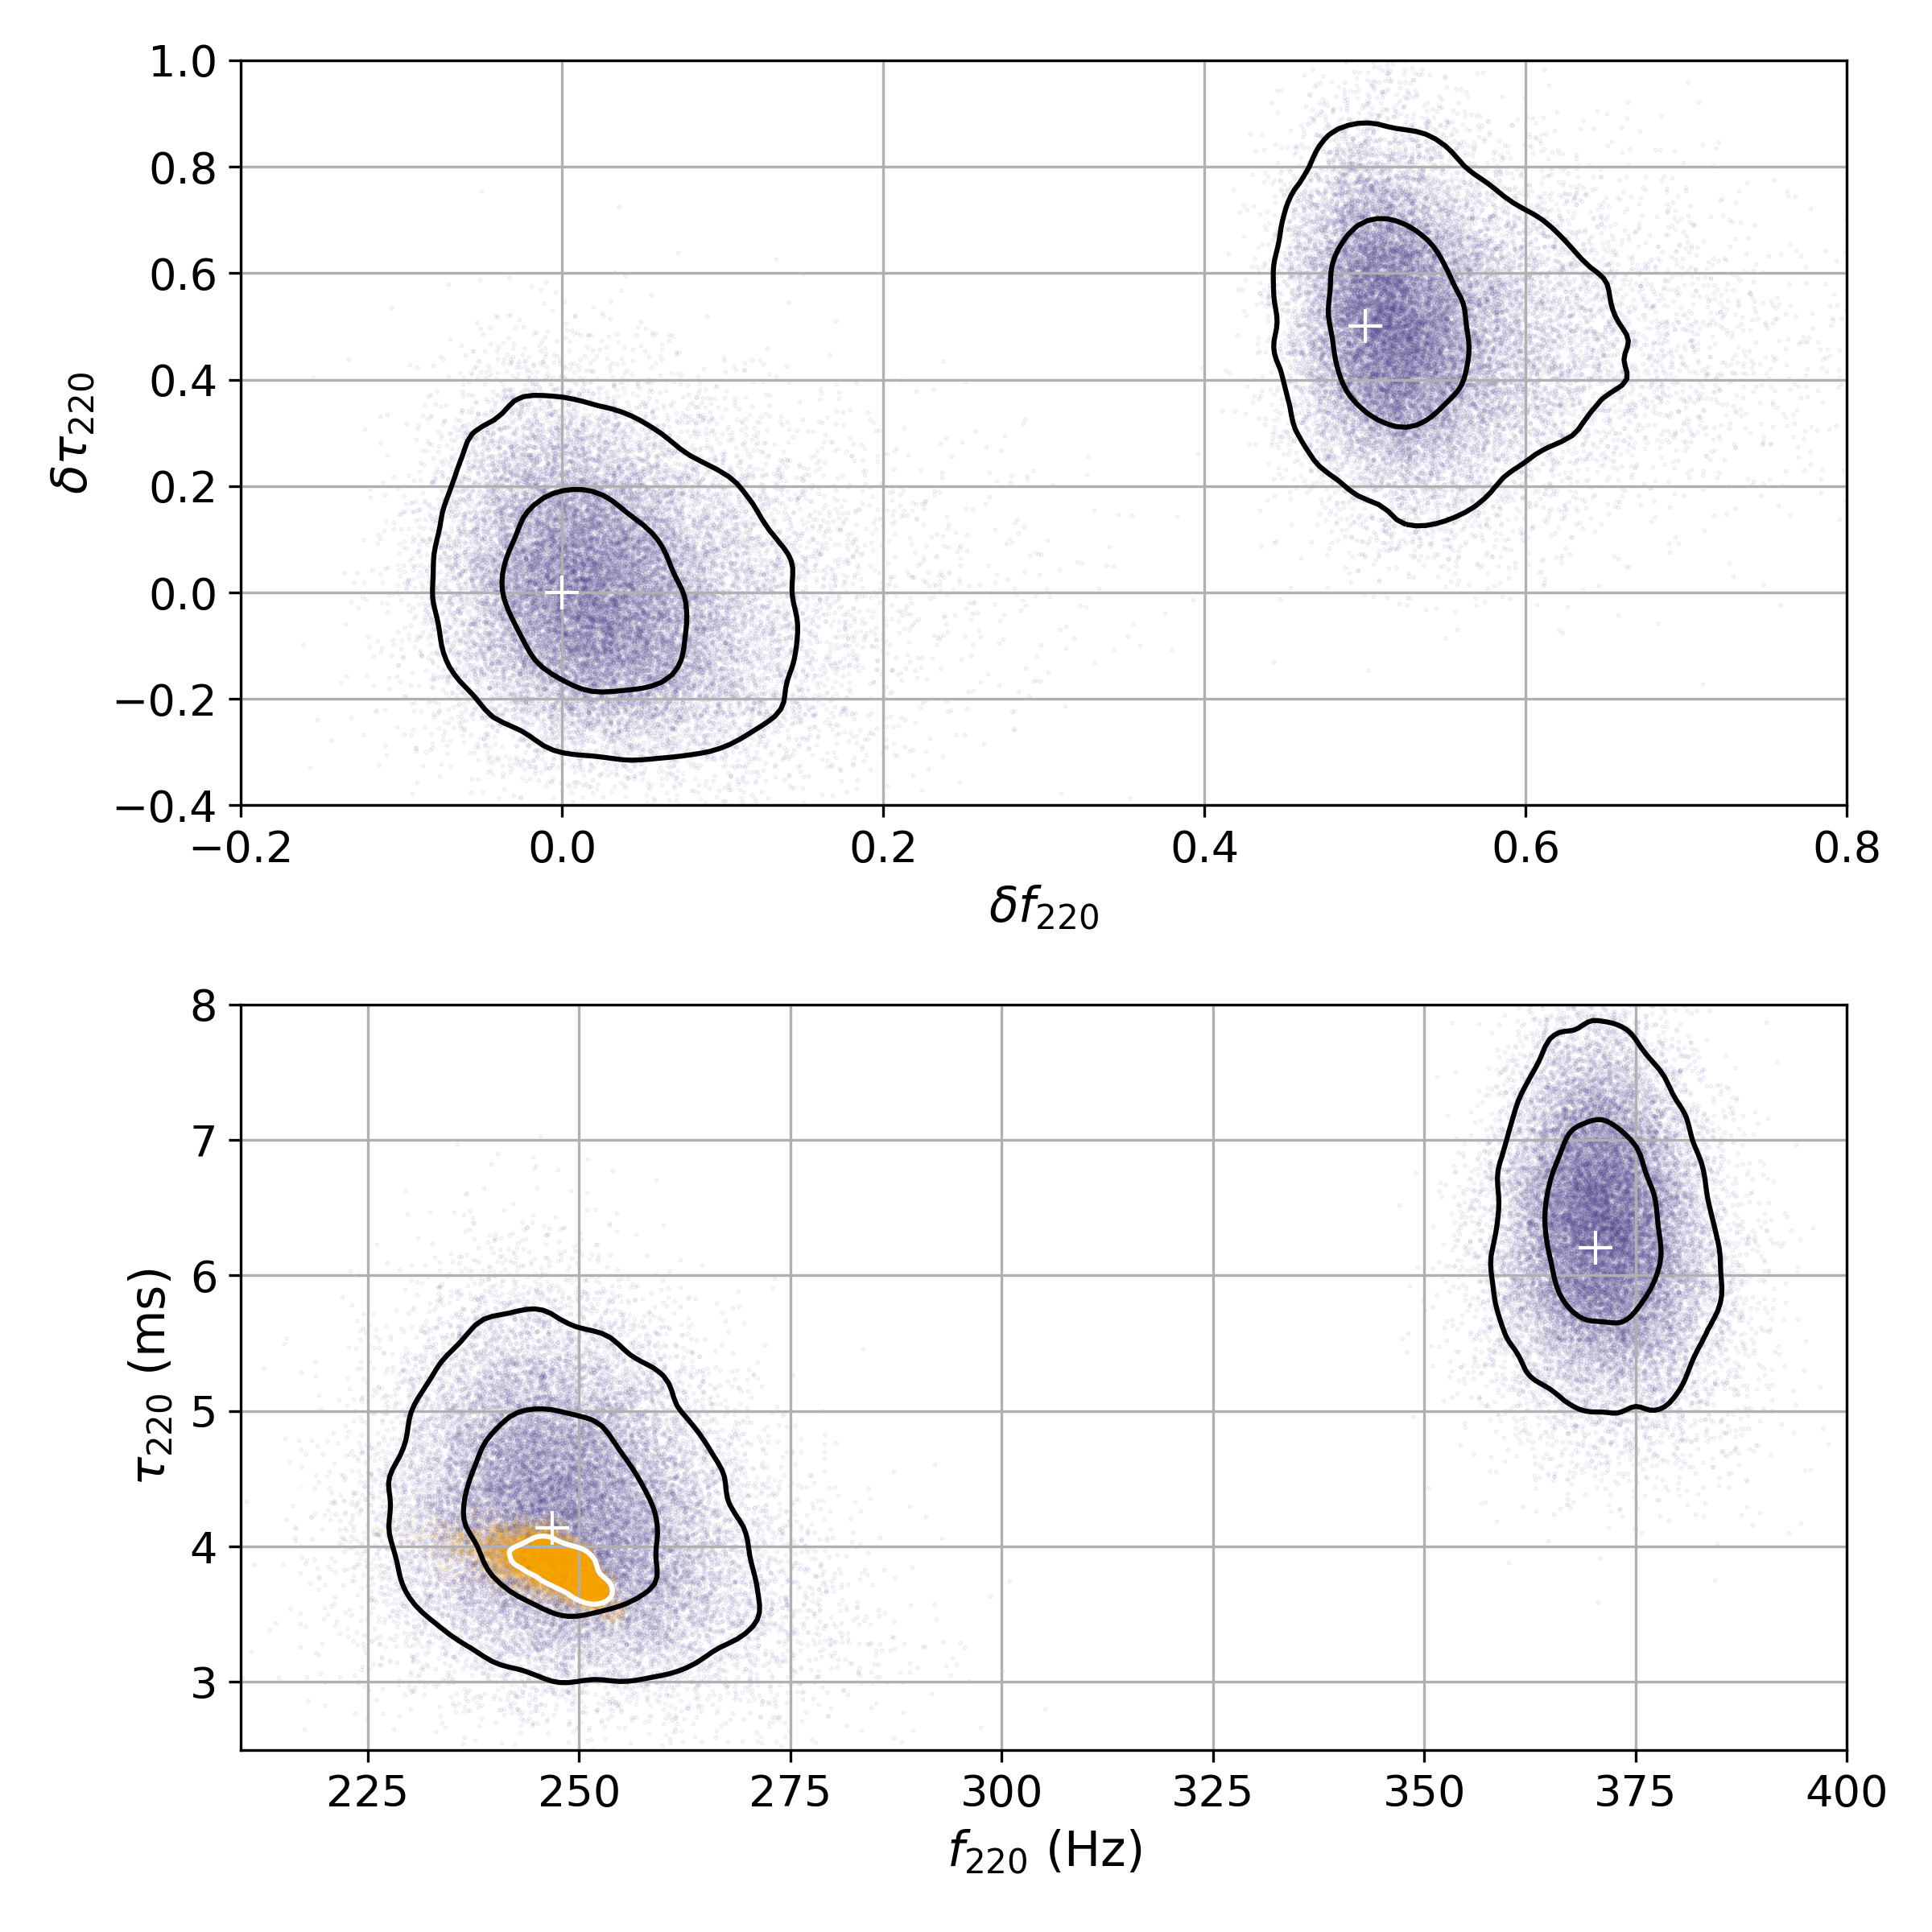
\includegraphics[width=0.5\textwidth]{figures/GW150914_simulated_signal_gr_ngr.png}
	\caption{\textcolor{red}{FINAL RESULT} Posterior probability distribution on the fractional deviations in the frequency and damping time of the $(2,2)$ QNM, $\{\df{220},\dtau{220}\}$ (top panel) and the reconstructed quantities, $(\fngr{220}, \taungr{220})$ (bottom panel) for an injection with initial parameters similar to GW150914 \ref{tab:injection_values}. The dark purple and grey points indicate the GR and modified GR signals respectively, when recovered using our $\pSEOB$ model. The two contours indicate the 50 and 90 \% credible levels, while the injected values are indicated by the '+' marker. The orange posterior probability distribution with the accompanying 90 \% credible level indicated in white corresponds to the biased measurement if our modGR signal had been estimated using the GR waveform model $SEOB$. }
	\label{fig:GW150914_simulated_signal}
\end{figure}
%%%%%%%%%%%%%%%%%%%%%%%%%%%%%%%%%%%%%%%%%%%%%%%%%%%%%%%%%%%%%%%
%%%%%%%%%%%%%%%%%%%%%%%%%%%%%%%%%%%%%%%%%%%%%%%%%%%%%%%%%%%%%%%

%%%%%%%%%%%%%%%%%%%%%%%%%%%%%%%%%%%%%%%%%%%%%%%%%%%%%%%%%%%%%%%
% GW190521-like simulated signal
%%%%%%%%%%%%%%%%%%%%%%%%%%%%%%%%%%%%%%%%%%%%%%%%%%%%%%%%%%%%%%%
\begin{figure}[h!]
	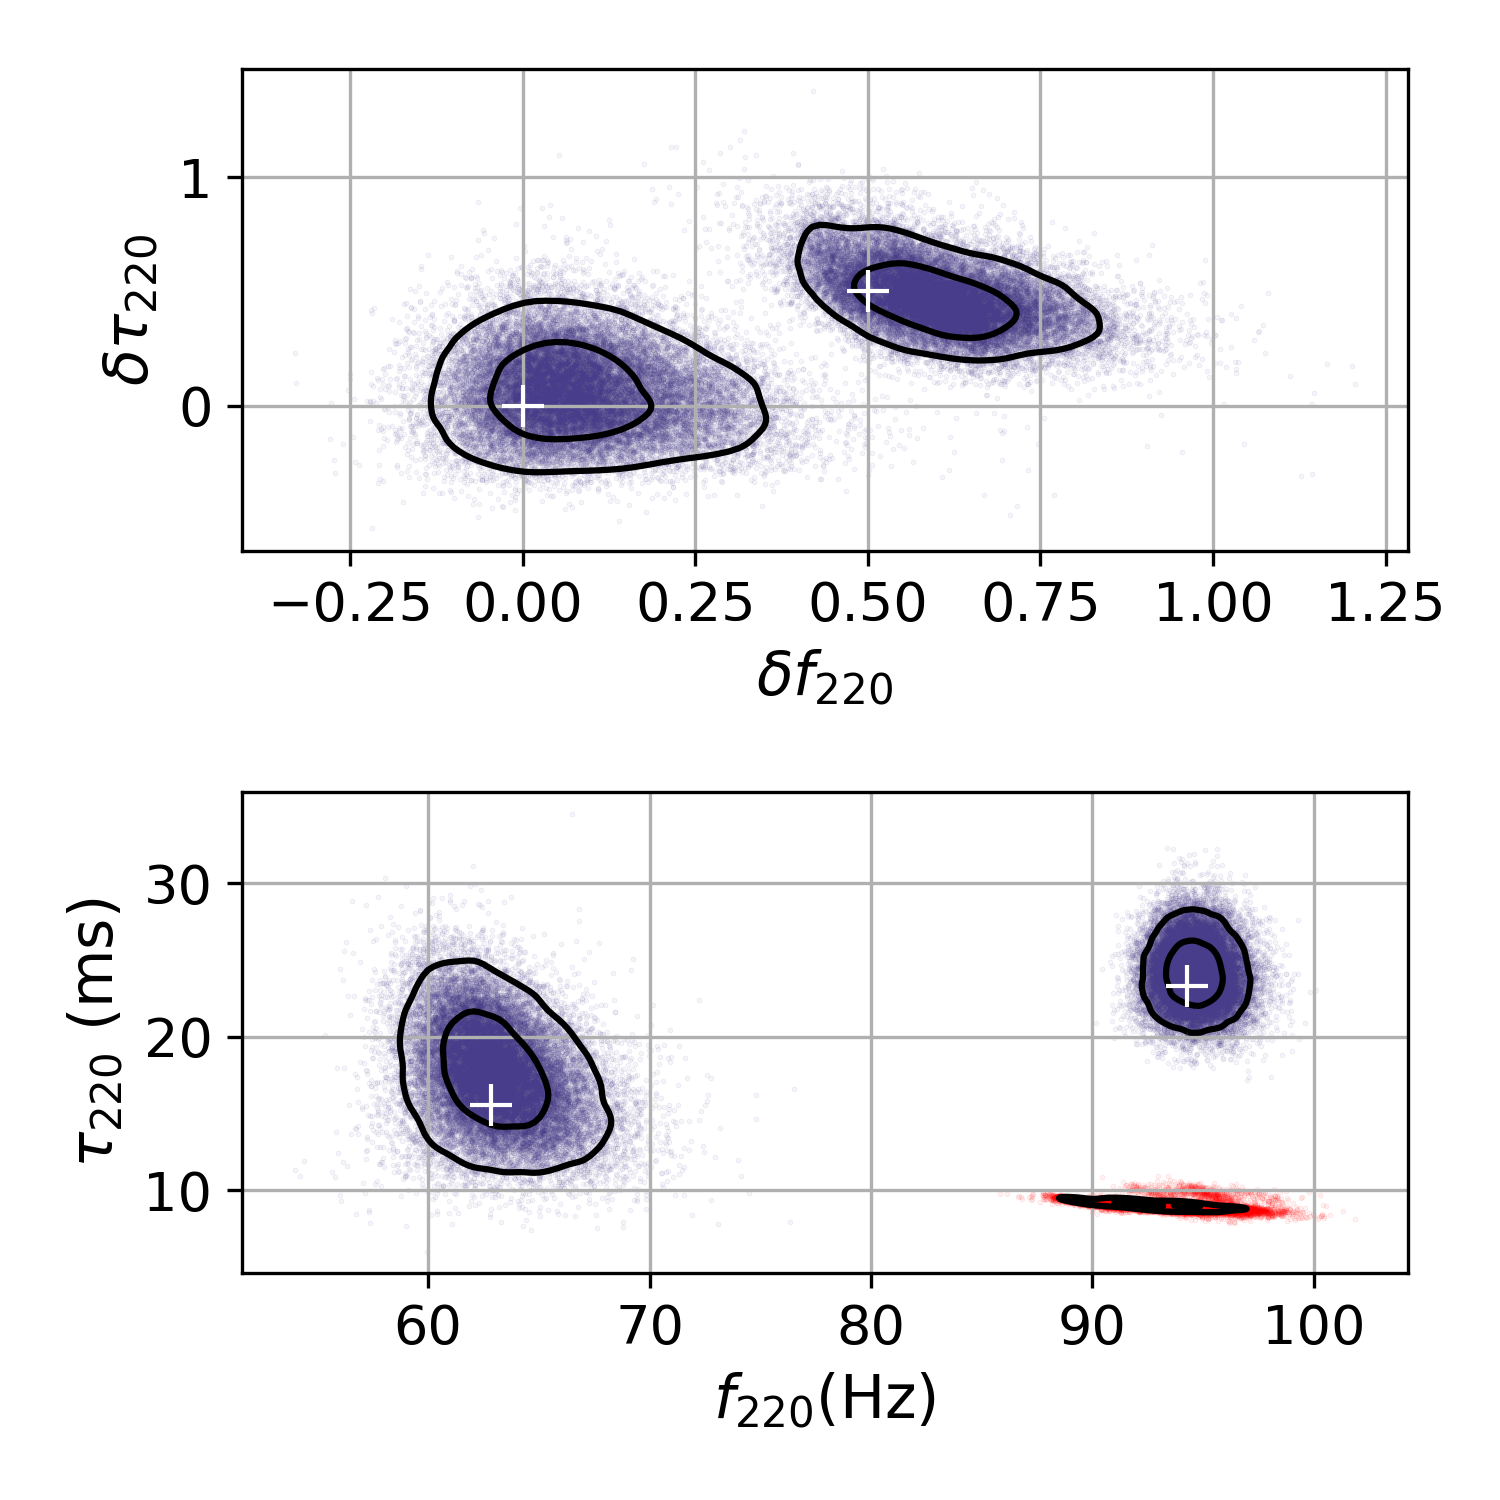
\includegraphics[width=0.5\textwidth]{figures/GW190521_simulated_signal_gr_ngr.png}
	\caption{\textcolor{red}{FINAL RESULT} Posterior probability distribution on the fractional deviations in the frequency and damping time of the $(2,2)$ QNM, $\{\df{220},\dtau{220}\}$ (top panel) and the reconstructed quantities, $(\fngr{220}, \taungr{220})$ (bottom panel) for an injection with initial parameters similar to GW190521 \ref{tab:injection_values}. The dark purple and grey points indicate the GR and modified GR signals respectively, when recovered using our $\pSEOB$ model. The two contours indicate the 50 and 90 \% credible levels, while the injected values are indicated by the '+' marker. The orange posterior probability distribution with the accompanying 90 \% credible level indicated in white corresponds to the biased measurement if our modGR signal had been estimated using the GR waveform model $SEOB$. }
	\label{fig:GW190521_simulated_signal}
\end{figure}
%%%%%%%%%%%%%%%%%%%%%%%%%%%%%%%%%%%%%%%%%%%%%%%%%%%%%%%%%%%%%%%
%%%%%%%%%%%%%%%%%%%%%%%%%%%%%%%%%%%%%%%%%%%%%%%%%%%%%%%%%%%%%%%

\iffalse
\abhi{The GW150914-like injections we have:}
\begin{itemize}
\item{an SEOBNRv4HM software injection with the 22 mode frequencies estimated}
\item{a non-spinning NR injection with parameters close to the real event but higher SNR for which 22 mode frequencies are estimated}
\item{a non-spinning highly-asymmetric (q=6) NR injection with total mass similar to GW150914 and high SNR for which 22 and 33 mode frequencies are estimated}
\end{itemize}
\fi


\subsection{Simulations using modified GR signals in Gaussian noise}

To demonstrate the robustness of the method in detecting possible deviations of the underlying GW signal from predictions of GR, we inject simulated GW signals which are identical to the corresponding GR prediction upto merger, and differ in their post-merger description. We again choose systems with initial-binary-parameters similar to GW150914 and GW190521, but we attach a phenomenological post-merger signal described by deviation parameters $\df{220} = \dtau{220} = 0.5$. In other words, we assume that the frequency and damping time of our non-GR signal is 1.5 times the corresponding GR prediction, although the pre-merger signal is identical to GR (Fig.\ref{fig:nongr_waveform}). We also avoid waveform and noise systematic biases by choosing a configuration identical to the simulations described in Sec.\ref{ssec:gr_signal}. The posterior probability distributions on $(\df{220}, \dtau{220})$ or equivalently $(\fngr{220}, \taungr{220})$ (right panels in Figs.\ref{fig:GW150914_simulated_signal} and \ref{fig:GW190521_simulated_signal}) are consistent with the corresponding the values of the injection parameters, indicated by plus signs. 

We additionally investigate the effects of erroneously assuming that an underlying modified GR signal can be well-described using GR. We do this by estimating the parameters of our modified GR signals using the GR waveform model $\SEOB$ instead of the parametrised $\pSEOB$. In such cases, we run the risk of biased pareameter estimates due to an incomplete understanding of the underlying signal. The resulting orange posterior probability distributions are shown in Figs.\ref{fig:GW150914_simulated_signal} and \ref{fig:GW190521_simulated_signal}) with the corresponding 90 \% credible level in white. The results are interesting and distinctly different for the two events. For the GW150914-like modified GR signal, the measurements of $(\fgr{220}, \taugr{220})$ (Fig.\ref{fig:GW150914_simulated_signal} lower panel) are consistent with the $(\fgr{220}, \taugr{220})$ measurements for a signal with no deviations. In other words, if the actual signal had deviations as large as the 50 \% of the GR prediction, the analysis with $\SEOB$ would likely have reported \emph{no} deviation from the GR prediction. However in the case of the GW190521-like modified GR signal, a simple GR analysis of the modified GR signal would have yielded measurements distinctly different from either of the two parametrised estimates: with and without deviations. The fact that the GW190521-like signal has a much lower SNR than GW150914 might be a possible reason for the the measurement of the final quantities to be more susceptible to noise.

%%%%%%%%%%%%%%%%%%%%%%%%%%%%%%%%%%%%%%%%%%%%%%%%%%%%%%%%%%%%%%%
%%%%%%%%%%%%%%%%%%%%%%%%%%%%%%%%%%%%%%%%%%%%%%%%%%%%%%%%%%%%%%%
\begin{figure}
	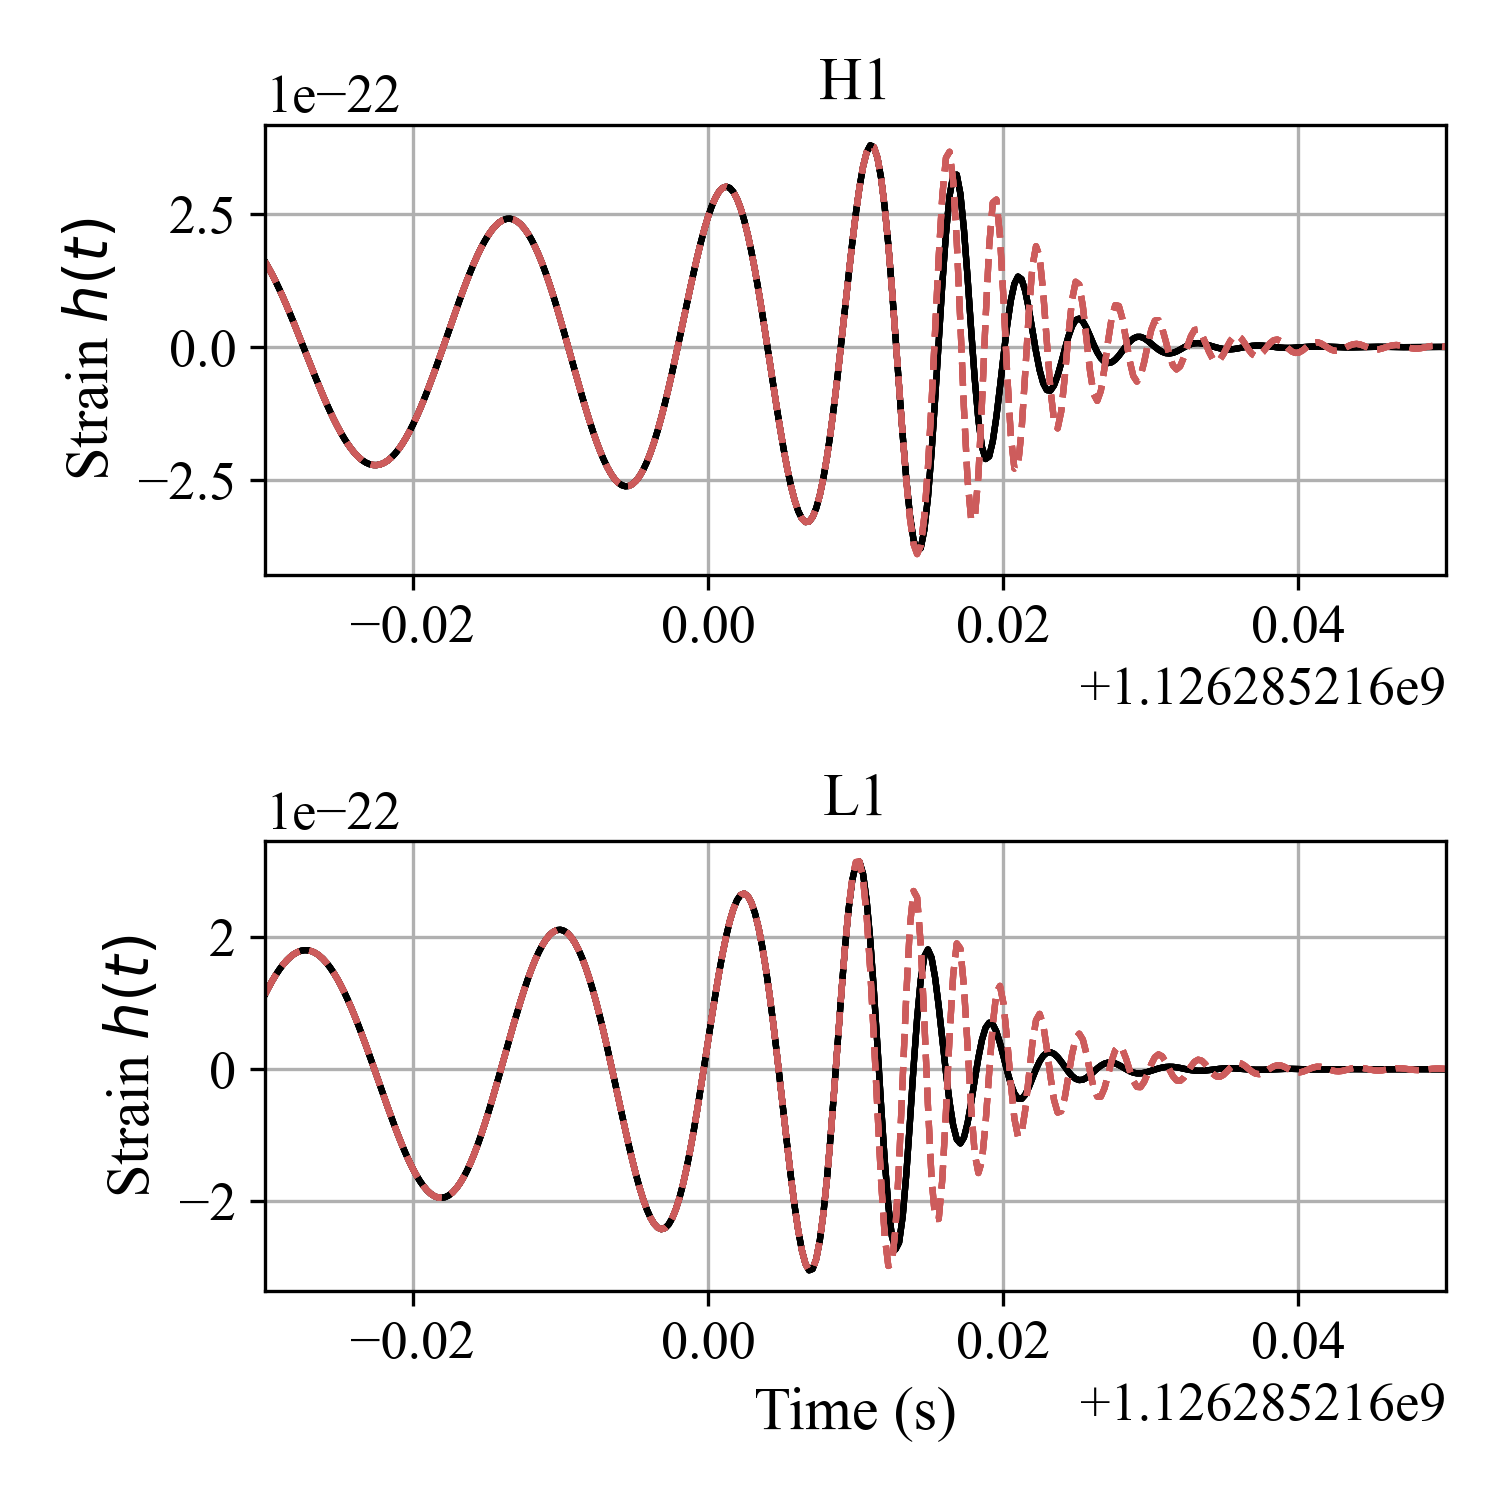
\includegraphics[width=0.5\textwidth]{figures/modGR_waveforms.png}
	\caption{\textcolor{red}{FINAL RESULT}The gravitational strain $h(t)$ in the LIGO Hanford (top panel) and Livingston (bottom panel) detectors, for a GW150914-like event where the ringdown is described by GR (black solid lines), i.e., $\df{220} = \dtau{220} = 0$, and where the ringdown frequencies are modified from GR (dashed red lines), i.e., $\df{220} = \dtau{220} = 0.5$. The time is measured with respect to UTC:1126285216, which was assumed to be point at which the event merged. The signals are identical up to merger, but show a distinctly different ringdown.}
	\label{fig:nongr_waveform}
\end{figure}
%%%%%%%%%%%%%%%%%%%%%%%%%%%%%%%%%%%%%%%%%%%%%%%%%%%%%%%%%%%%%%%
%%%%%%%%%%%%%%%%%%%%%%%%%%%%%%%%%%%%%%%%%%%%%%%%%%%%%%%%%%%%%%%

\subsection{Test of the No hair theorem}\label{ssec:nohairtheorem}

Finally, we provide a simple demonstration of a test of the no-hair theorem using our model. As described in the introduction, any test of the no-hair theorem of black holes would need to involve independent measurements of (at least) two different QNMs. We use a simulated GW signal from the SXS catalog CITE corresponding a non-spinning binary black hole with a mass-ratio $q=6$ (SXS:BBH:0166), rescaled to a total mass of $M=84 \Mo$. We choose an asymmetric system to increase the SNR in the higher modes. We also rescale the distance and orientation of the binary such that the total SNR of the signal in a network of three detectors, LIGO Hanford, Livingston and Virgo, is 75. The LIGO detectors are assumed to be in the ZDHP configuration as before, while the Virgo detector is assumed to be at design sensitivity CITE. Based on the LIGO-Virgo observations during O3a, such asymmetric and loud signals are no longer just a theoretical prediction but quite plausible at design sensitivities. Using the signal, we attempt to measure the QNM frequencies $(2,\pm 2)$ and $(3,\pm 3)$ modes together (Fig.~\ref{fig:nohair_sxs}). The fractional deviations in the estimates of the damping time and frequency of either mode is expected to be consistent with 0, as we indeed find in the left panel of Fig.~\ref{fig:nohair_sxs}. Consequently we find that the reconstructed quantities $(\fngr{220}, \taungr{220})$ and $(\fngr{330}, \taungr{330})$  are also consistent with the corresponding predictions for a BBH merger in GR. As a consequence, the information from these two independent measures correspond to a unique remnant object, which is completely described by its mass and spin angular momentum. For most of the events observed so far, the power in the $(3,\pm 3)$ has not been sufficient to measure it along with the $(2,\pm 2)$, or in fact, in its place. However, it might also be possible to combine information from multiple observation, as is likely over the coming few years of gravitational wave astronomy with the LIGO-Virgo detectors, to obtain meaningful constraints on the $(3,\pm 3)$ and other sub-dominant QNMs.

%%%%%%%%%%%%%%%%%%%%%%%%%%%%%%%%%%%%%%%%%%%%%%%%%%%%%%%%%%%%%%%

%%%%%%%%%%%%%%%%%%%%%%%%%%%%%%%%%%%%%%%%%%%%%%%%%%%%%%%%%%%%%%%
\begin{figure}
	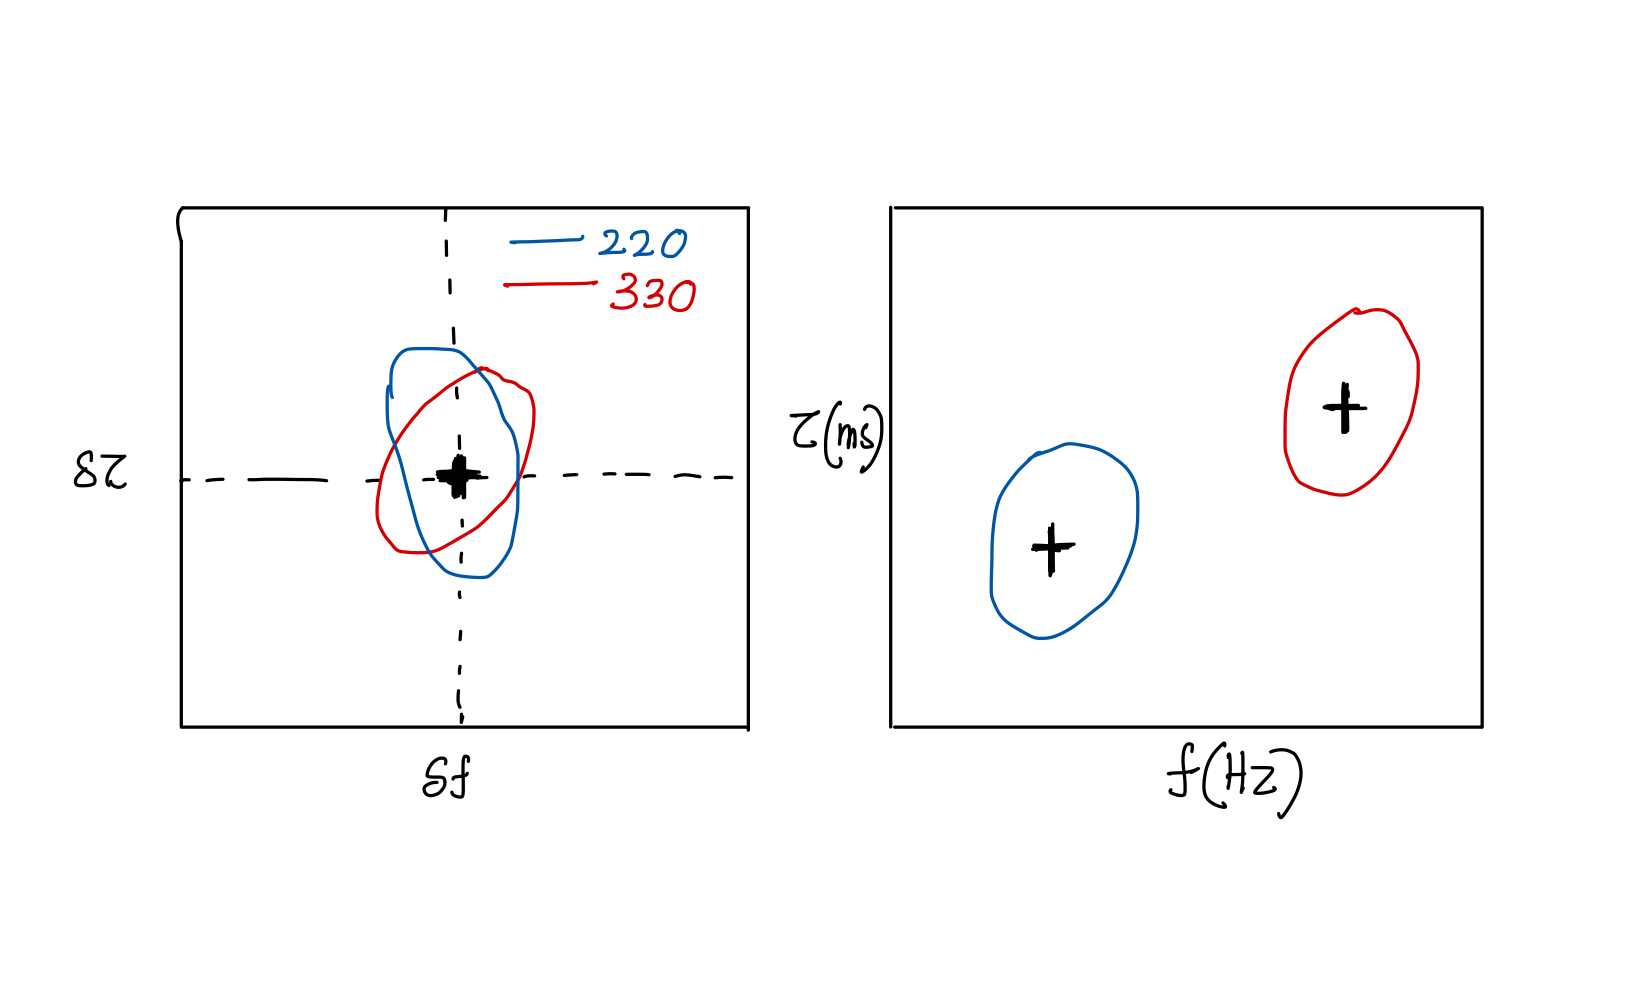
\includegraphics[width=0.5\textwidth]{figures/nohair_sxs_0166_placeholder.png}	
	\caption{\textcolor{red}{DEMO FIGURE; RUN ONGOING} Posterior probability distribution on the fractional deviations (left panel) and the reconstructed (right panel) frequency and damping time of the $(2,\pm 2)$ (blue curves) and $(3,\pm 3)$ (red curves) respectively, for a numerical relativity signal corresponding to a BBH merger of $q=6$,  $M=84 \Mo$ and SNR $75$. The plus signs mark the GR predictions.}
	\label{fig:nohair_sxs}
\end{figure}
%%%%%%%%%%%%%%%%%%%%%%%%%%%%%%%%%%%%%%%%%%%%%%%%%%%%%%%%%%%%%%%
%%%%%%%%%%%%%%%%%%%%%%%%%%%%%%%%%%%%%%%%%%%%%%%%%%%%%%%%%%%%%%%

\subsection{Results on actual LIGO-Virgo results}

The LIGO-Virgo Collaboration recently released their testing GR catalogue containing results of this test for all events observed during the first half of O3 CITE, which passed a threshold for the total detector frame mass $\geq 50 \Mo$ and SNRs in the pre- and post-merger regions $\geq 8$.The pre- and post-merger regions of the signal are identified as the power in the frequency content of the signal before and after the signal reaches peak amplitude, as determined by the maximum likelihood parameter estimation template. We restricted ourselves to the high-mass events which are expected to be merger-ringdown dominated. However, since our method relies on doing a parameter estimation on the entire inspiral-merger-ringdown signal, we require the SNR to be beyond a certain threshold throughout the signal for reliable parameter estimation of the initial and final quantities. Fig.~\ref{fig:o1o2_events} contains three events from O3a, GW190519\_ 153544, GW190521\_ 074359, GW190910\_ 112807.

For the first time, in this paper, we present results on the relevant events from LIGO-Virgo's first and second observing runs, alongside the above events. Applying the same thresholds as above, we find three additional events which could be included in the analysis: GW150914, GW170104, GW170729 \abhi{would need to confirm the thresholds again, and see if GW170809 qualifies}. Regarding the other two high-mass events, GW170814 and GW170823 do not satisfy the SNR thresholds. For the three relevant signals, GW150914, GW170104 and GW170729, we provide the posterior distributions in $(\df{220}, \dtau{220})$ in Fig.\ref{fig:o1o2_events}. We also reconstruct the effective QNM parameters, $(\fngr{220}, \taungr{220})$ which are tabulated in Table~\ref{tab:qnm_o1o2_results}. 

Among all the GW signals detected so far, GW150914 is unique in its loudness, mass as well as the clarity of the signal, leading to the first, and to date, best attempt in measuring the QNM frequencies CITE.  Fig.\ref{fig:GW150914_real} compares the results we obtain for GW150914 using $\pSEOB$ with previously published LIGO-Virgo results using a damped-sinusoid method, as well as the measurement reported using a non-spinning model in \paperone. The damped-sinusoid model assumed specific cutoff times (indicated in the curves on the bottom panel of Fig.\ref{fig:o1o2_events}) after the time corresponding to the peak amplitude as predicted by the best-fitting GR template waveform. Increasing time, decreasing SNR, wider posteriors, less-precise measurement. Compared to that we see when we incorporate the complete IMR version of the test, we utilise more SNR leading to tighter constraints.

%%%%%%%%%%%%%%%%%%%%%%%%%%%%%%%%%%%%%%%%%%%%%%%%%%%%%%%%%%%%%%%
% O1-O2 events
%%%%%%%%%%%%%%%%%%%%%%%%%%%%%%%%%%%%%%%%%%%%%%%%%%%%%%%%%%%%%%%
\begin{figure}[h!]
	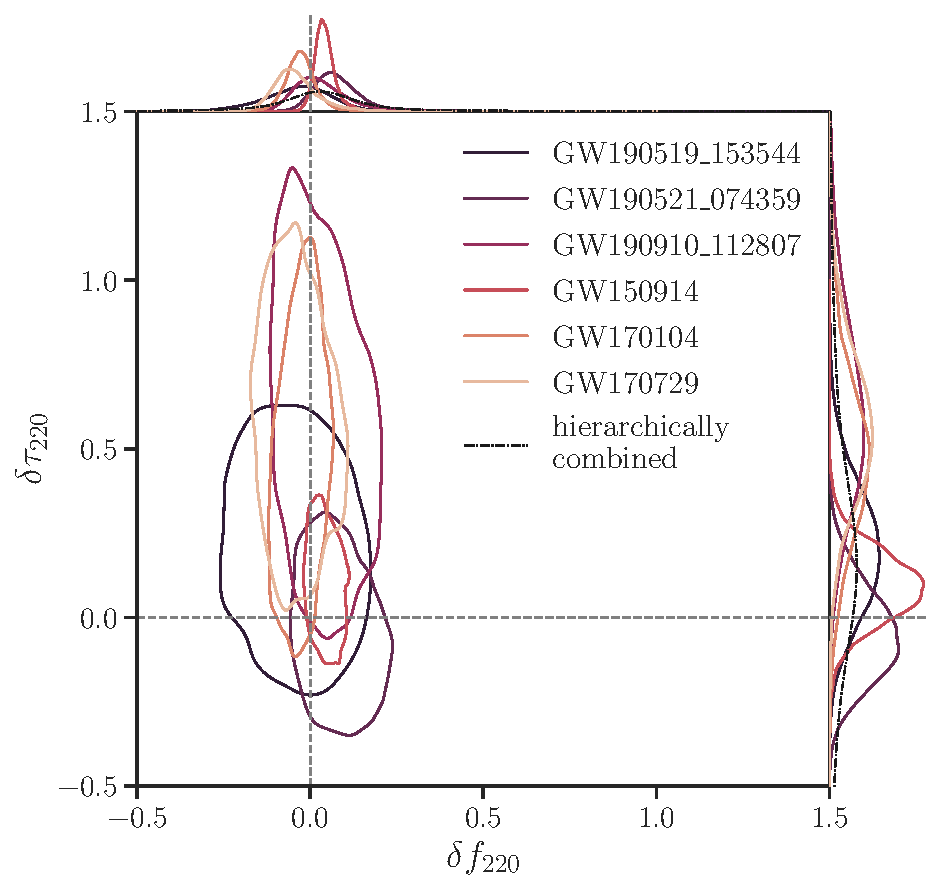
\includegraphics[width=0.5\textwidth]{figures/O1O2_realevents.pdf}
	\caption{\textcolor{red}{FINAL RESULT}The 90\% credible levels of the posterior probability distribution of the fractional deviations in the frequency and damping time of the $(2,\pm 2)$ QNM, $\{\df{220},\dtau{220}\}$ and their corresponding one-dimensional marginalized posterior distributions. We also plot the joint probability distribution obtained by multiplying the likelihoods of the $\{\df{220},\dtau{220}\}$ (black dashed line) \abhi{need to compute the joint likelihood. currently contains the hierarchical contour from the O3a TGR paper}}
	\label{fig:o1o2_events}
\end{figure}
%%%%%%%%%%%%%%%%%%%%%%%%%%%%%%%%%%%%%%%%%%%%%%%%%%%%%%%%%%%%%%%
%%%%%%%%%%%%%%%%%%%%%%%%%%%%%%%%%%%%%%%%%%%%%%%%%%%%%%%%%%%%%%%

%%%%%%%%%%%%%%%%%%%%%%%%%%%%%%%%%%%%%%%%%%%%%%%%%%%%%%%%%%%%%%%
% GW150914
%%%%%%%%%%%%%%%%%%%%%%%%%%%%%%%%%%%%%%%%%%%%%%%%%%%%%%%%%%%%%%%
\begin{figure}[h!]
	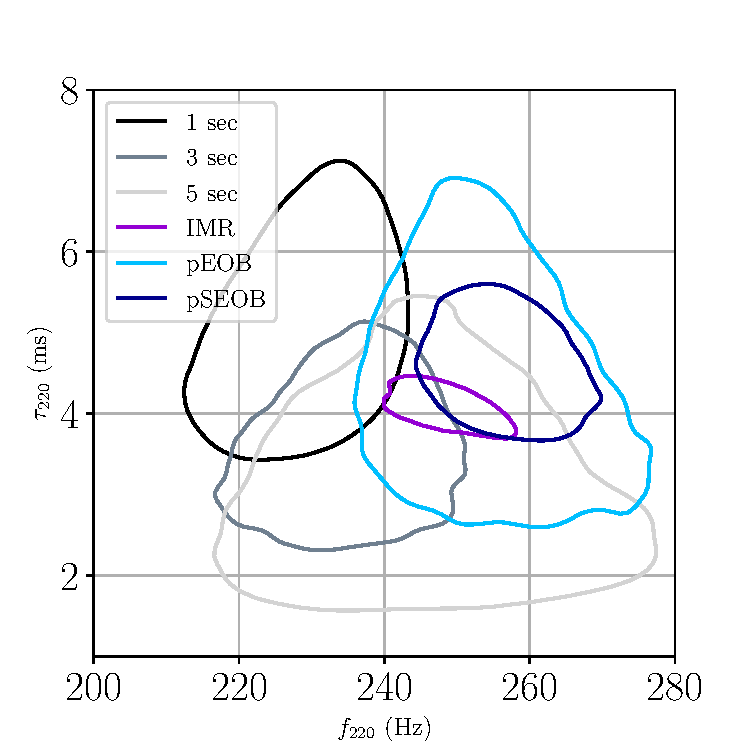
\includegraphics[width=0.4\textwidth]{figures/GW150914.pdf}
	\caption{\textcolor{red}{FINAL RESULT}The 90\% credible levels of the posterior probability distribution of the frequency and damping time of the $(2,2)$ QNM for GW150914. The measurements by fitting damped sinusoids to the signal 1,3,5 milli-seconds after the peak amplitude is given by the black, darkgrey and grey curves. The measurement using NR fits is the purple contour, while the $\pSEOB$ and $pEOB$ measurements are indicated by the dark blue and light blue contours respectively.}
	\label{fig:GW150914_real}
\end{figure}
%%%%%%%%%%%%%%%%%%%%%%%%%%%%%%%%%%%%%%%%%%%%%%%%%%%%%%%%%%%%%%%
%%%%%%%%%%%%%%%%%%%%%%%%%%%%%%%%%%%%%%%%%%%%%%%%%%%%%%%%%%%%%%%


Finally, if we assume that the fractional deviations $(\df{220}, \dtau{220})$ take the same values in multiple events, we can assume the posterior of one event to be the prior for the next, and obtain a joint posterior probability distribution. For $N$ observations, where $P_j(\df{220}, \dtau{220} | d_j)$ is the posterior for the $j-th$ observation corresponding to the data set $d_j$, $j=1...N$, the joint posterior is given by:
\begin{equation}
P(\df{220}, \dtau{220} | \{d_j\}) = P(\df{220}, \dtau{220}) \prod _{j=1}^N \frac{P(\df{220}, \dtau{220} | d_j) }{P(\df{220}, \dtau{220})}
\end{equation}
where $P(\df{220}, \dtau{220})$ is the prior on $(\df{220}, \dtau{220})$. However, since we assume the prior on $(\df{220}, \dtau{220})$ to be flat or uniform, the joint posterior is equal to the joint likelihood.

We show these joint likelihoods on $(\df{220}, \dtau{220})$, as well as the corresponding one-dimensional marginalised distributions as black dashed lines in Fig.~\ref{fig:o1o2_events}. These are the strongest constraints on possible deviations in the measurement of $(\df{220}, \dtau{220})$ to date using our method. \abhi{perhaps show 2 joint posteriors: only O3a and O3a+O1-O2 to explicitly show the tightening of the joint constraints by adding the O1-O2 events}

\begin{table}
\begin{center}
\begin{tabular}{llllllll}
\toprule
Event & \multicolumn{2}{c}{Redshifted} & \hphantom{X} & \multicolumn{2}{c}{Redshifted} \\
& \multicolumn{2}{c}{frequency [Hz]} & \hphantom{X} & \multicolumn{2}{c}{damping time [ms]} \\[0.075cm]
\cline{2-4}
\cline{6-8}
& IMR  & pSEOB & \hphantom{X} & IMR  & pSEOB \\
\midrule

GW150914 &
$249^{+9}_{-7}$ &
$-$ &
\hphantom{X} &
$4.1^{+0.3}_{-0.2}$ &
$-$
\\[0.075cm]

GW170104 &
$286^{+16}_{-27}$ &
$-$ &
\hphantom{X} &
$3.5^{+0.4}_{-0.3}$ &
$-$
\\[0.075cm]

GW170729 &
$161^{+13}_{-14}$ &
$-$ &
\hphantom{X} &
$7.8^{+1.8}_{-1.5}$ &
$-$
\\[0.075cm]

\bottomrule
\end{tabular}
\caption{\textcolor{red}{NOT COMPLETE}}
\label{tab:qnm_o1o2_results}
\end{center}
\end{table}

\section{Discussion}\label{sec:discussion}

\iffalse
\abhi{A comparison with pyRING}
\abhi{damped sinusoid results}
\fi

\pagebreak

\appendix
\section{Study of noise syetematics on ringdown measurements}\label{sec:noise_systematics}

\iffalse
\abhi{A small summary of the noise systematics study that was done for S190521g to show that the deviations seen were consistent with systematics due to noise. The study include 2 separate sections: in Gaussian noise, and in real LIGO-Virgo noise immediately adjacent to the actual event.}
\fi

In order to investigate the 

%%%%%%%%%%%%%%%%%%%%%%%%%%%%%%%%%%%%%%%%%%%%%%%%%%%%%%%%%%%%%%%
%%%%%%%%%%%%%%%%%%%%%%%%%%%%%%%%%%%%%%%%%%%%%%%%%%%%%%%%%%%%%%%
\begin{figure}
	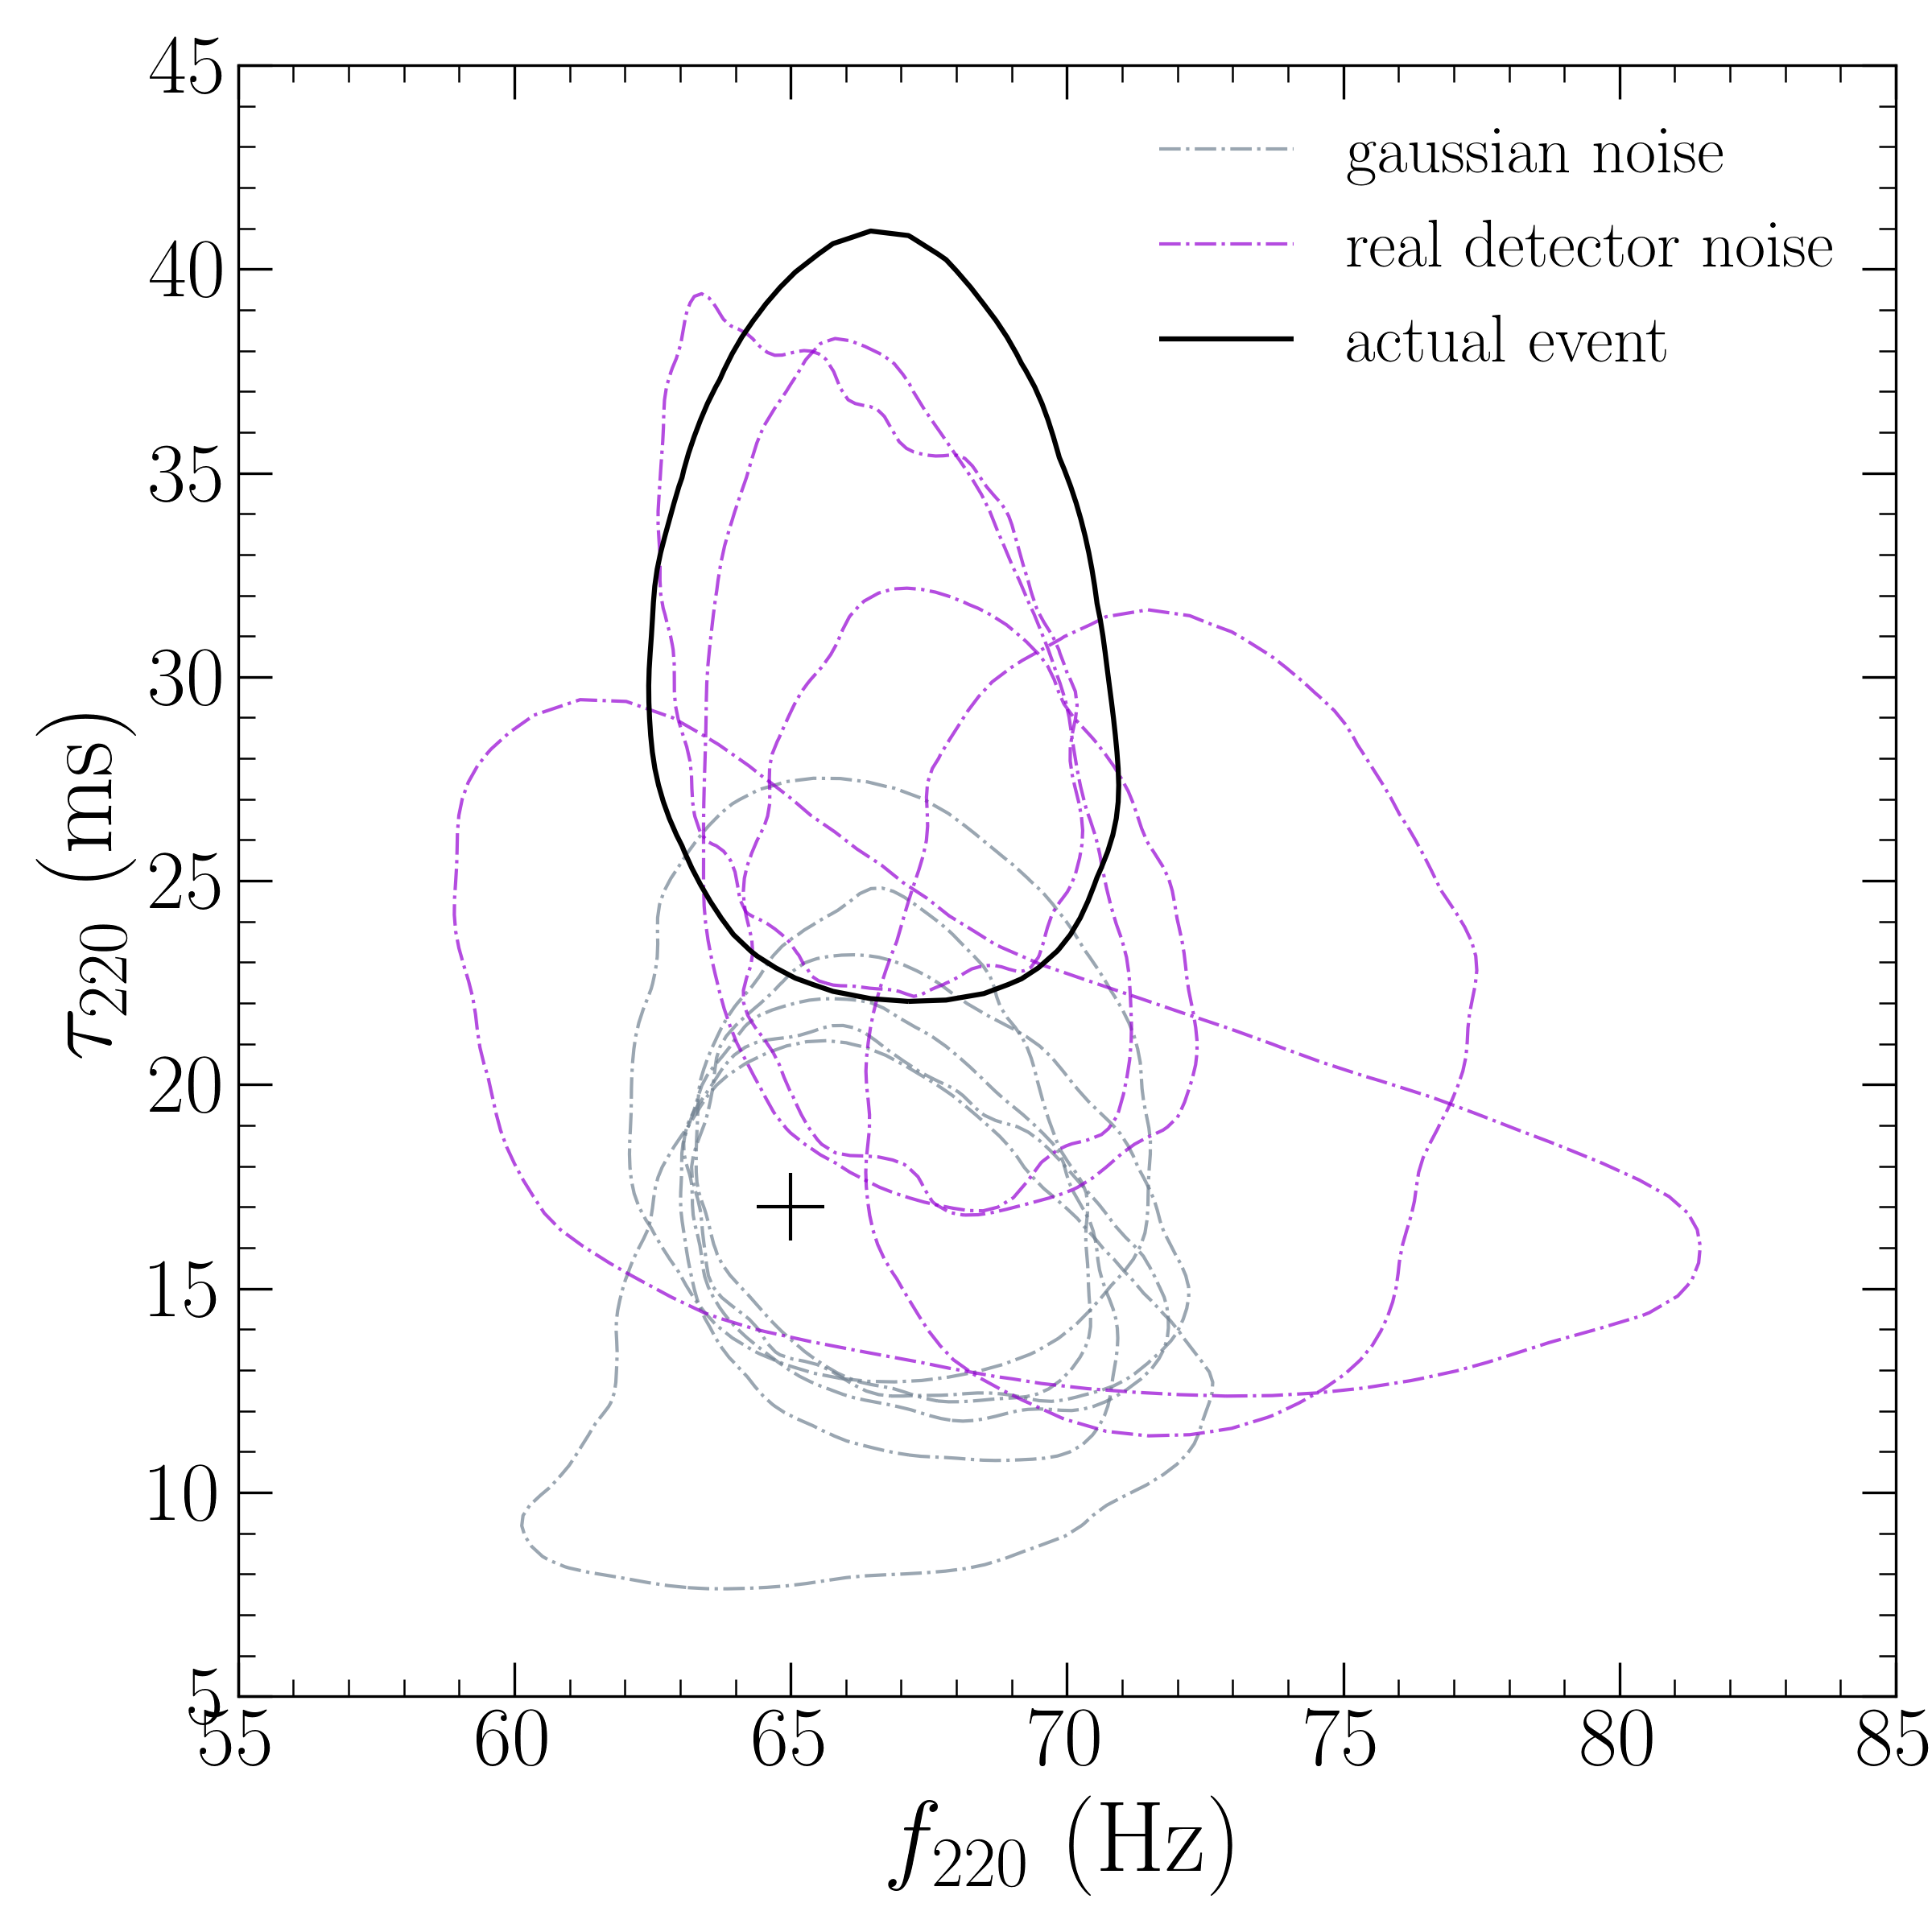
\includegraphics[width=0.4\textwidth]{figures/S190521g_swinjs.png}
	\caption{\textcolor{red}{FINAL RESULT}90 \% credible level on the posterior probability distribution of the frequency and damping time of $(2,\pm 2)$ mode, $(\fgr{220}, \taugr{220}$ from simulations of an \texttt{NRSur7dq4} GW signal with parameters similar to the GW event, GW190521, in Gaussian noise (grey dot-dashed lines) and real interferometric noise (pink dot dashed lines). The GR prediction for the frequency and damping time is indicated by the black cross. While the Gaussian noise simulations are consistent with the prediction, at least 3 or the 5 real noise simulation are not. For comparison, we also plot the 90 \% credible level for the actual event, GW190521.}
	\label{fig:21g_systematics}
\end{figure}
%%%%%%%%%%%%%%%%%%%%%%%%%%%%%%%%%%%%%%%%%%%%%%%%%%%%%%%%%%%%%%%
%%%%%%%%%%%%%%%%%%%%%%%%%%%%%%%%%%%%%%%%%%%%%%%%%%%%%%%%%%%%%%%

We injected NRSur7dq4 signal using the MaxL parameters from EXP30, in 2.5 hours of data surrounding the event at: t0-1.5 hours, t0-1., t0-0.5, t0+0.5, t0+1. For 3 of the 5 noise realisations, corresponding to t0-1 hour, t0+0.5 hours, and t0+1.0 hour we recover a damping time similar to the actual event, whereas for a third case, t0-0.5 hours, we obtain a damping time consistent at the 90\% credible interval (bottom panel of FIg.\ref{fig:21g_systematics}). L1-SNR goes down by more than 3 in some runs (maximum L1-SNR 12, minimum 9), indicative of how the noise variability is strongly affecting the recovered parameters. For some injections the mass ratio is biased, although final spin (most sensitive to mass ratio) is not affected much.  domega varies quite a lot among runs, instead dtau seems well behaved around zero. Effective frequency is a stable parameter (always well measured), while effective tau is much more sensitive to the noise configuration.  


%%%%%%%%%%%%%%%%%%%%%%%%%%%%%%%%%%%%%%%%%%%%%%%%%%%%%%%%%%%%%%%
% GW190521-like simulated GR signal: corner plot
%%%%%%%%%%%%%%%%%%%%%%%%%%%%%%%%%%%%%%%%%%%%%%%%%%%%%%%%%%%%%%%
\begin{figure*}[h!]
	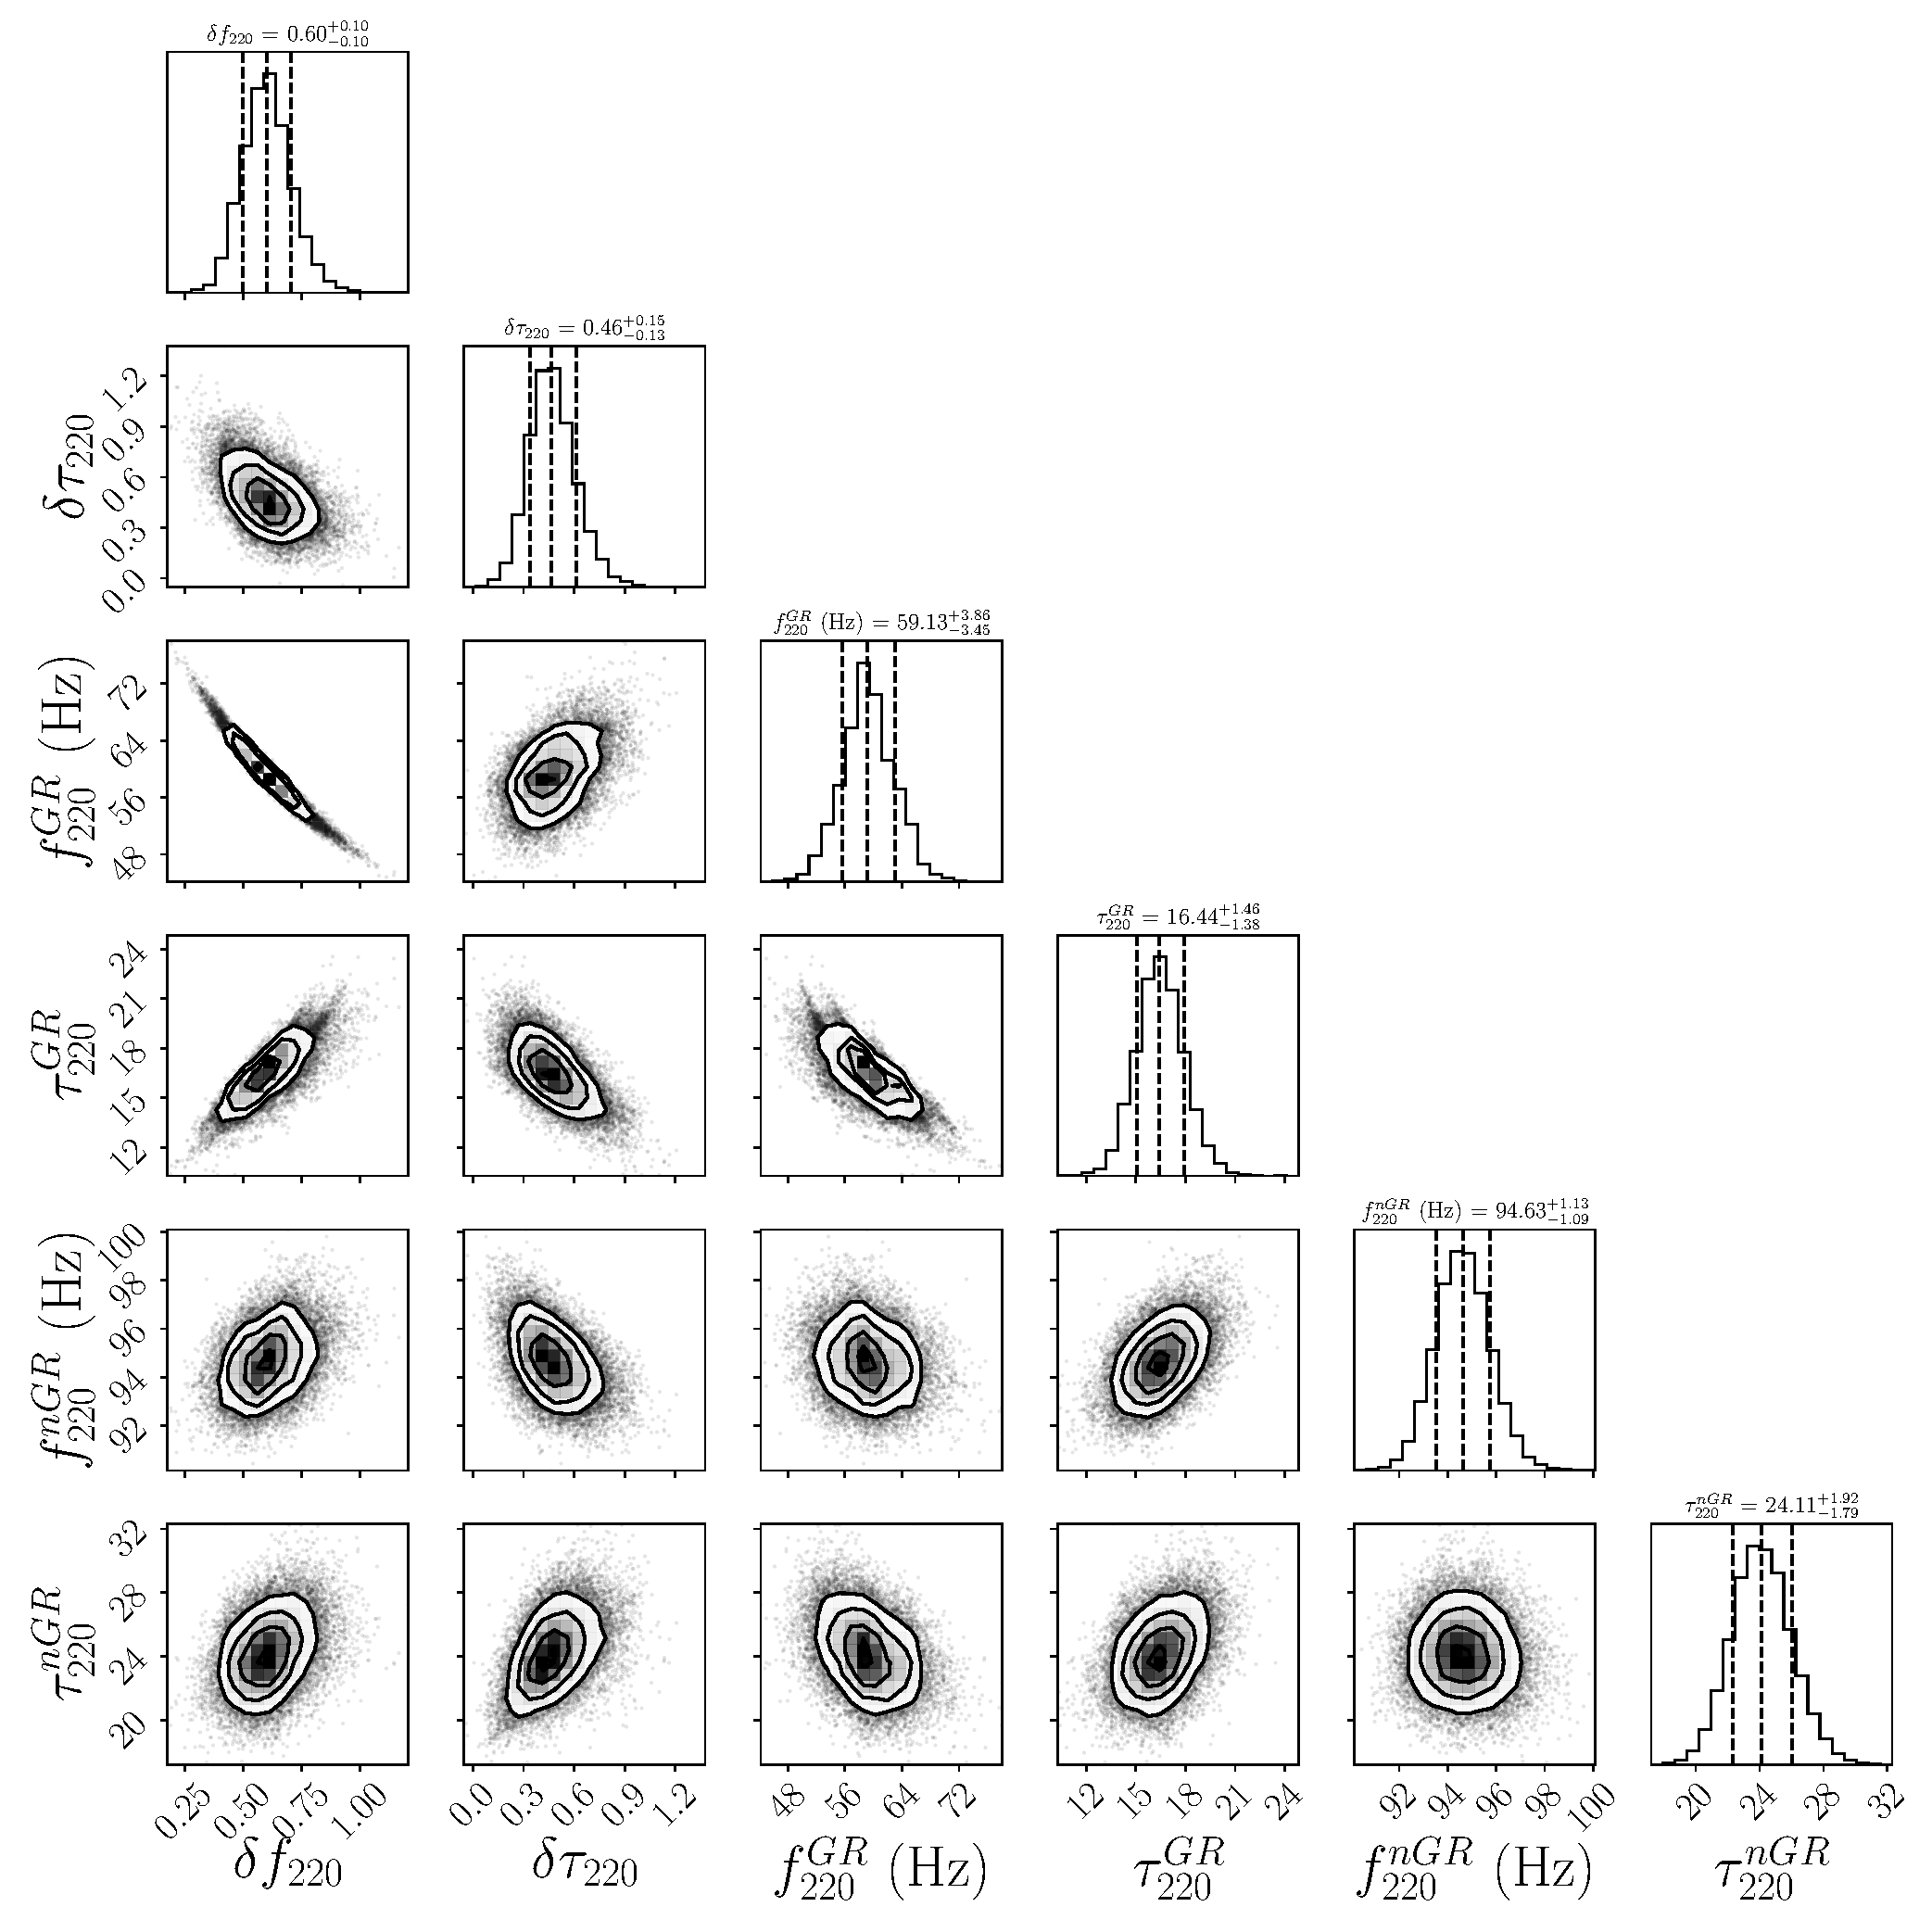
\includegraphics[width=\textwidth]{figures/GW190521_simulated_signal_gr_corner.pdf}
	\caption{\textcolor{red}{FINAL RESULT} Corner plot showing the two-dimensional posterior probability distributions and corresponding one-dimensional marginalised distributions of the fractional deviations in the frequency and damping time of the $(2,\pm 2)$ QNM, i.e, $(\df{220}, \dtau{220})$,  the GR predictions $(\fgr{220}, \taugr{220})$ and the reconstructed quantities $(\fngr{220}, \taungr{220})$ for a GW190521-like simulated GR signal. The dashed lines on the one-dimensional marginalised histograms correspond to the median and the 90 \% confidence intervals of the distribution.}
	\label{fig:GW190521_simulated_GR_signal_corner}
\end{figure*}
%%%%%%%%%%%%%%%%%%%%%%%%%%%%%%%%%%%%%%%%%%%%%%%%%%%%%%%%%%%%%%%
%%%%%%%%%%%%%%%%%%%%%%%%%%%%%%%%%%%%%%%%%%%%%%%%%%%%%%%%%%%%%%%


%
\bibliographystyle{apsrev}
\bibliography{intro_paper}

\end{document}